% Provenance (never printed): see sources/outline_sources.md (Year 1: elastic rebound and the
% seismic cycle; seismic moment and magnitudes; focal mechanisms; geodetic measurement of
% active deformation; the Gutenberg--Richter law). Exercise and problem values in the Book 3
% scratch calculator calc/ch18.py; figure data from figdata/bachelor-1/gutenberg_richter.py,
% beachballs.py and interseismic.py. Focus, epicentre, magnitude, intensity and seismometer
% are owned by Book 1 g7 (magnitude re-founded here as the moment magnitude); P and S waves by
% Book 2 g11; fault types and rake by ch. 17; stress, Coulomb and the seismogenic layer by
% ch. 16; the shear modulus by physics. Radar interferometry and the stereographic projection
% belong to later volumes (told, not defined).
\chapter{भूकंप का उद्गम}\label{ch:b1:earthquake-source}

% ledger: pp1515:1906, reid:1910
18 अप्रैल 1906 की सुबह, सैन फ़्रांसिस्को के उत्तर और दक्षिण की ज़मीन चार सौ किलोमीटर से अधिक लंबी एक रेखा के साथ फट गई। इस रेखा को पार करने वाली सड़कें, बाड़ें और पेड़ों की पंक्तियाँ कट गईं, और हर एक के दो भाग मीटरों दूर पाए गए, पश्चिमी भाग हमेशा उत्तर की ओर विस्थापित। सर्वेक्षकों ने पिछली आधी सदी में इस क्षेत्र के भू-चिह्नों की स्थितियाँ मापी थीं, और जब उन्हें फिर से मापा गया तो तुलना ने भंजन से भी अधिक अजीब बात दिखाई: भूकंप से पहले दशकों तक ज़मीन धीरे और सहजता से मुड़ रही थी, और भूकंप ने उसे वापस उछलने दिया। यह अध्याय एक भूकंप को भ्रंश के धीमे भार से लेकर उन कुछ मिनटों तक अनुसरित करता है जिनमें वह सरकता है, और सरकन को तरंगों और ज़मीन से वापस पढ़ता है: वह कितना बड़ा था, किस दिशा में खिसका, अगला कितनी तेज़ी से तैयार हो रहा है, और हर आकार के भूकंप कितनी बार आते हैं।

\begin{recall}
भूकंप का उद्गम वह बिंदु है जहाँ भंजन शुरू होता है, और उसका अधिकेंद्र उसके ऊपर सतह का बिंदु; परिमाण भूकंप के आकार को मापता है, तीव्रता किसी स्थान पर कंपन को; एक भूकंपमापी ज़मीन की गति को भूकंपलेख के रूप में दर्ज करता है (पुस्तक~1, कक्षा~7)। P तरंग, जो संपीडन-तरंग है, पहले पहुँचती है, और S तरंग, जो कर्तन-तरंग है, उसके बाद (पुस्तक~2, कक्षा~11)। एक भ्रंश की एक \omterm{def:b1:faults-folds-fabrics:fault-elements}{लटकती दीवार} और एक \omterm{def:b1:faults-folds-fabrics:fault-elements}{पादभित्ति} होती है; \omterm{def:b1:faults-folds-fabrics:fault-elements}{सरकन-सदिश} \omterm{def:b1:faults-folds-fabrics:fault-elements}{लटकती दीवार} का \omterm{def:b1:faults-folds-fabrics:fault-elements}{पादभित्ति} के सापेक्ष \omterm{def:b1:cross-sections:throw}{विस्थापन} है, उसका \omterm{def:b1:faults-folds-fabrics:fault-elements}{रेक} $r$ भ्रंश-तल पर \omterm{def:b1:geological-maps:attitude}{स्ट्राइक} से मापा जाता है, और \omterm{def:b1:faults-folds-fabrics:fault-elements}{रेक} भ्रंश का नाम देता है: लगभग \ang{90} उत्क्रम, लगभग \ang{-90} सामान्य, लगभग 0 \omterm{def:b1:faults-folds-fabrics:fault-types}{बाएँ-पार्श्वीय}, लगभग \ang{180} \omterm{def:b1:faults-folds-fabrics:fault-types}{दाएँ-पार्श्वीय} (\cref{ch:b1:faults-folds-fabrics})। एक प्रत्यास्थ ठोस प्रतिबल हटाने पर अपना आकार वापस पाता है; कर्तन मापांक $\mu$ एक कर्तन प्रतिबल को उससे उत्पन्न कर्तन विकृति से जोड़ता है (भौतिकी की पुस्तकें); भ्रंश तब सरकते हैं जब कर्तन प्रतिबल उनकी घर्षण-सामर्थ्य तक पहुँचता है, और भूकंप \omterm{def:b1:layered-earth:layers}{भूपर्पटी} के भंगुर ऊपरी भाग में शुरू होते हैं, \omterm{def:b1:stress-strain-rheology:strength-envelope}{भूकंप-जनक परत} में (\cref{ch:b1:stress-strain-rheology})। उपग्रह-स्थिति निर्धारण के स्थायी स्टेशन, जिनकी वर्षों की दैनिक स्थितियाँ उस स्थान पर ज़मीन का वेग देती हैं जहाँ वे खड़े हैं, प्लेटों की गति मापते हैं (\cref{ch:b1:plate-kinematics})।
\end{recall}

\section{प्रत्यास्थ प्रतिक्षेप और भूकंपीय चक्र}\label{sec:b1:earthquake-source:cycle}

स्थिर दर से एक-दूसरे के पास से सरकती दो प्लेटें सामान्यतः अपने बीच के भ्रंश के साथ स्थिरता से नहीं सरकतीं। घर्षण भ्रंश को अवरुद्ध रखता है जबकि प्लेटें उससे दूर चलती रहती हैं, इसलिए दोनों ओर की चट्टानें एक स्प्रिंग की तरह मुड़ती हैं। जब भ्रंश पर कर्तन प्रतिबल उसकी सामर्थ्य तक पहुँचता है, तो भ्रंश कुछ सेकंड या मिनटों में सरकता है, और मुड़ी चट्टानें झटके से वापस लौटती हैं।

\begin{definition}[प्रत्यास्थ प्रतिक्षेप, भूकंपीय चक्र, पुनरावृत्ति अंतराल]
\label{def:b1:earthquake-source:seismic-cycle}
\emph{प्रत्यास्थ प्रतिक्षेप}\index{प्रत्यास्थ प्रतिक्षेप} वह अचानक वापसी है जिसमें भ्रंश के दोनों ओर की चट्टानें अपने अविकृत आकार की ओर लौटती हैं, जब भ्रंश, जो उनके विकृत होने के दौरान अवरुद्ध था, एक भूकंप में सरकता है; उनमें संचित प्रत्यास्थ ऊर्जा मुक्त होती है, जिसका कुछ भाग भूकंपीय तरंगों के रूप में। किसी भ्रंश-खंड का \emph{भूकंपीय चक्र}\index{भूकंपीय चक्र} एक लंबी अंतर-भूकंपीय अवस्था का बार-बार दोहराया क्रम है, जिसमें खंड अवरुद्ध रहता है और उसके चारों ओर विकृति जमा होती है; एक सह-भूकंपीय अवस्था, यानी भूकंप, जिसमें वह सरकता है; और एक पश्च-भूकंपीय अवस्था, महीनों से दशकों तक, जिसमें आसपास का भाग नई अवस्था के अनुरूप समायोजित होता है। किसी खंड का \emph{पुनरावृत्ति अंतराल}\index{पुनरावृत्ति अंतराल} उस पर दो क्रमागत बड़े भूकंपों के बीच का समय है।
\end{definition}
% ledger: usgs:gloss-rebound, reid:1910, usgs:pp1515-thatcher

\begin{omfigure}
\begin{tikzpicture}[>={Stealth[length=5pt]}, font=\small]
% map view of a fence across a locked dextral strike-slip fault (north up): (a) built straight;
% (b) after decades of loading, bent with the interseismic profile v(x) = -(s/pi) arctan(x/D)
% (dextral: the east side moves south); (c) after the earthquake, straight again on each side and
% offset by s at the fault. Panel 3.4 cm wide (x from -1.7 to 1.7 cm), D = 0.35 cm, s = 0.9 cm.
\def\s{0.9}\def\Dl{0.35}
\foreach \k/\t in {0/{(a) बाड़ बनाई गई}, 1/{(b) दशकों का भार}, 2/{(c) भूकंप के बाद}} {
  \begin{scope}[xshift=\k*4.6cm]
    \fill[omLithSand!25] (-1.7,-1.6) rectangle (1.7,1.6);
    \draw[black!50, line width=0.4pt] (-1.7,-1.6) rectangle (1.7,1.6);
    \draw[fault, line width=1.1pt] (0,-1.6) -- (0,1.6);
    \node[anchor=north, align=center, font=\scriptsize] at (0,-1.7) {\t};
    % far-field motion of the two blocks, relative to the fault
    \draw[->, omThm, line width=0.8pt] (-1.35,-1.25) -- (-1.35,-0.45);
    \draw[->, omThm, line width=0.8pt] (1.35,1.25) -- (1.35,0.45);
    \ifnum\k=0
      \draw[line width=1.2pt, omDef] (-1.7,0) -- (1.7,0);
    \fi
    \ifnum\k=1
      \draw[line width=1.2pt, omDef] plot[domain=-1.7:1.7, samples=81, variable=\x] (\x, {-\s/pi*atan(\x/\Dl)*pi/180});
      \draw[black!45, dashed, line width=0.4pt] (-1.7,0) -- (1.7,0);
    \fi
    \ifnum\k=2
      \draw[line width=1.2pt, omDef] (-1.7,{\s/2}) -- (0,{\s/2});
      \draw[line width=1.2pt, omDef] (0,{-\s/2}) -- (1.7,{-\s/2});
      \draw[black!45, dashed, line width=0.4pt] (-1.7,0) -- (1.7,0);
      \draw[<->, line width=0.5pt] (0.18,{\s/2}) -- (0.18,{-\s/2});
      \node[anchor=west, font=\scriptsize] at (0.2,0.12) {सरकन};
    \fi
  \end{scope}
}
\node[anchor=south, font=\scriptsize] at (0,1.62) {भ्रंश};
\draw[->, line width=0.5pt] (-1.5,0.75) -- (-1.5,1.15) node[above, font=\scriptsize, inner sep=1pt] {\omnameCompassN};
\end{tikzpicture}
\par\smallskip{\small बाड़ पर ऊपर से देखा गया \omterm{def:b1:earthquake-source:seismic-cycle}{प्रत्यास्थ प्रतिक्षेप}, जो एक अवरुद्ध \omterm{def:b1:faults-folds-fabrics:fault-types}{दाएँ-पार्श्वीय} भ्रंश के आर-पार सीधी बनाई गई है (नीली बाड़)। लाल तीर: भ्रंश से दूर, दोनों खंडों की गति, भ्रंश के सापेक्ष। (b) जब भ्रंश अवरुद्ध है, दूर की ज़मीन चलती है और बाड़ मुड़ती है, अंतर-भूकंपीय परिच्छेद के वक्र के अनुसार जो \cref{sec:b1:earthquake-source:geodesy} में है। (c) भूकंप मोड़ को मुक्त करता है: बाड़ का हर आधा भाग फिर सीधा है, और दोनों आधे भ्रंश पर सरकन जितने विस्थापित हैं। मोड़ बढ़ा-चढ़ाकर दिखाया गया है: एक वास्तविक बाड़ दसियों किलोमीटर पर कुछ मीटर मुड़ती है।}
\label{fig:b1:earthquake-source:rebound}
\end{omfigure}

यदि भ्रंश भूकंपों के बीच अवरुद्ध है और हर भूकंप उस सरकन को उलट देता है जो प्लेटों ने पिछले भूकंप के बाद जमा की, तो प्लेट की गति चक्र की गति तय करती है।

\begin{proposition}[पुनरावृत्ति से सरकन-दर तक]
\label{prop:b1:earthquake-source:recurrence}
मान लीजिए एक भ्रंश-खंड दीर्घकालिक सरकन-दर $\dot s$ पर भारित है, भूकंपों के बीच अवरुद्ध है, और हर भूकंप में उतना ही सरकन $D$ करता है। तब उसके भूकंपों का \omterm{def:b1:earthquake-source:seismic-cycle}{पुनरावृत्ति अंतराल}
\[
  T = \frac{D}{\dot s} .
\]
यदि सरकन-दर का केवल भाग $c$ अवरुद्ध है, और शेष बिना भूकंपों के स्थिर रूप से सरकता है, तो $T = D/(c\,\dot s)$।
\end{proposition}

\begin{proof}
दीर्घ समय $t$ में, भ्रंश की दोनों ओर एक-दूसरे के सापेक्ष $\dot s\,t$ विस्थापित होती हैं। भ्रंश से दूर ज़मीन स्थिरता से चलती है, इसलिए भ्रंश पर स्वयं वही विस्थापन पूरा होना चाहिए, यहाँ केवल भूकंपों से: यदि $N$ भूकंप समय $t$ में हुए, तो एक भूकंप के सरकन तक $N D = \dot s\,t$, और $t/N \to D/\dot s$। सरकन के भाग $1-c$ के स्थिर फिसलन से होने पर, भूकंप $c\,\dot s\,t$ की पूर्ति करते हैं, और $t/N \to D/(c\,\dot s)$।
\end{proof}

\qty{4}{m} प्रति महा-भूकंप के सरकन और \qty{20}{mm.yr^{-1}} के सरकन-दर वाले सैन एंड्रियास भ्रंश के विशिष्ट मानों के साथ, \omterm{def:b1:earthquake-source:seismic-cycle}{पुनरावृत्ति अंतराल} \qty{200}{yr} है। मध्य कैलिफ़ोर्निया में वैलेस क्रीक पर, भ्रंश को आर-पार काटने वाली एक जलधारा-नाली उसके उत्कीर्ण होने के बाद से \num{3587} वर्षों में \qty{128}{m} विस्थापित हुई है, औसतन \qty{36}{mm.yr^{-1}}, जो वहाँ अन्य विस्थापनों पर मापी गई लगभग \qty{34}{mm.yr^{-1}} की दर के निकट है; उस खंड पर अंतिम महा-भूकंप, 1857 में, लगभग \qty{10}{m} सरका था, जिसे इस दर पर जमा होने में लगभग तीन सदियाँ लगेंगी।
% ledger: usgs:pp1515-thatcher, usgs:pp1515-wallace, commons:wallace-creek

\begin{omfigure}
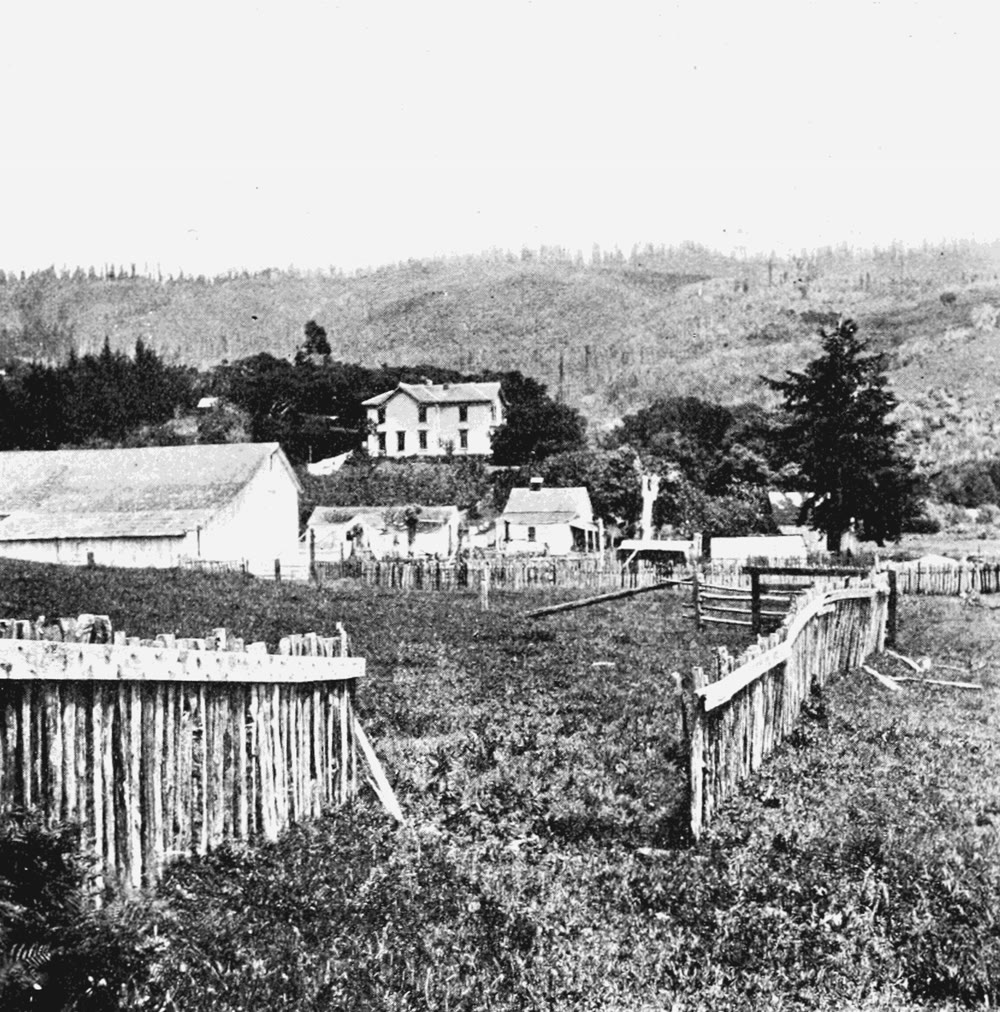
\includegraphics[height=5.6cm]{images/book3/b1-fence-1906.jpg}\hfill
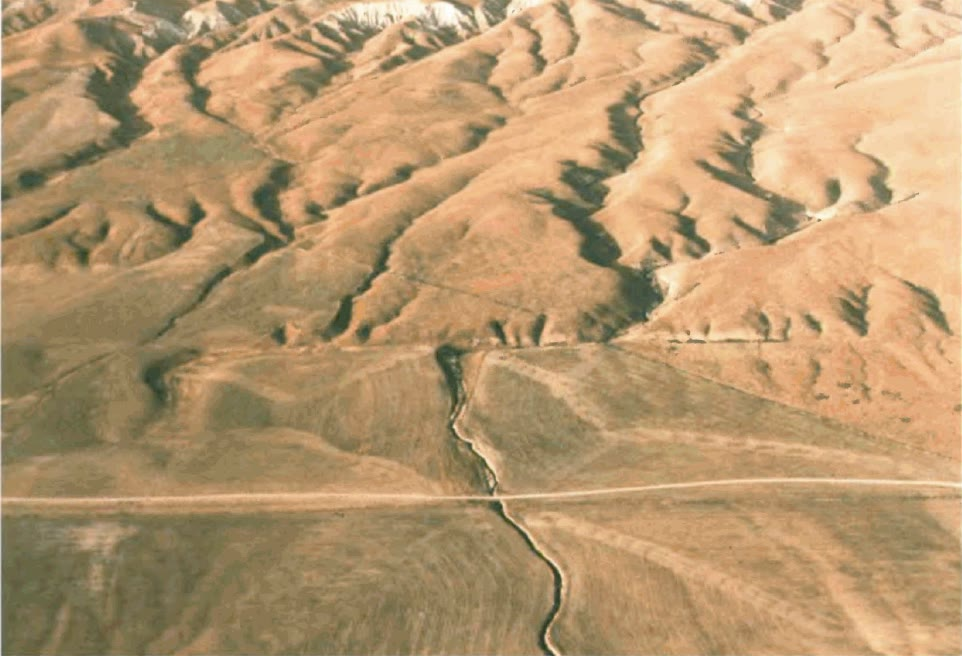
\includegraphics[height=5.6cm]{images/book3/b1-wallace-creek.jpg}
\par\smallskip{\small बाएँ: मारिन काउंटी में, सैन फ़्रांसिस्को के उत्तर में, खेतों की बाड़ें, जिन्हें 1906 के भंजन ने काटा, उसी वर्ष प्रकाशित, ``भूकंपीय भ्रंश से अलग हुई ज़मीन'' के शीर्षक से। फ़ोटो: \emph{Popular Science Monthly}, खंड~69 (1906), सार्वजनिक क्षेत्र। दाएँ: कैरिज़ो मैदान पर वैलेस क्रीक, हवाई से देखा गया: जलधारा पहाड़ियों से नीचे आती है (ऊपर), और जहाँ वह सैन एंड्रियास भ्रंश को पार करती है, पहाड़ियों के तल पर, उसकी नाली \qty{130}{m} तिरछी खिसक गई है, वह विस्थापन जो हज़ारों वर्षों के भूकंपों में जमा हुआ। फ़ोटो: R.~E.~Wallace, U.S. Geological Survey, सार्वजनिक क्षेत्र। दोनों विकिमीडिया कॉमन्स से।}
\label{fig:b1:earthquake-source:offsets}
\end{omfigure}
% ledger: commons:psm-fence, commons:wallace-creek

अनुमान एक औसत देता है, समय-सारणी नहीं। उसी भ्रंश पर पार्कफ़ील्ड के निकट, 1857 में लगभग \num{6} परिमाण का एक भूकंप, \qty{30}{km} के उसी खंड पर उसके बाद, लगभग 22 वर्षों के अंतराल पर, 1966 तक, पाँच और, उनके जैसे ही, आए; अगला 1993 से पहले अपेक्षित था, और 2004 में आया, \num{6.0} \omterm{def:b1:earthquake-source:mw}{आघूर्ण परिमाण} के साथ और बिना किसी स्पष्ट चेतावनी-चिह्न के। किसी भ्रंश की सामर्थ्य, हर भूकंप का सरकन, और उसके पड़ोसियों से भार, सब एक चक्र से दूसरे चक्र तक बदलते हैं, और \omterm{def:b1:earthquake-source:seismic-cycle}{भूकंपीय चक्र} को एक माध्य \omterm{def:b1:earthquake-source:seismic-cycle}{पुनरावृत्ति अंतराल} और उसके चारों ओर के प्रसार से, किसी आवर्तकाल से अधिक, बेहतर वर्णित किया जाता है।
% ledger: pp1515:parkfield, bl85:parkfield, usgs:hist-mw, bakun:2005

कुछ भ्रंश-खंड बिल्कुल अवरुद्ध नहीं होते। पार्कफ़ील्ड और सैन जुआन बॉतिस्ता के बीच, सैन एंड्रियास भ्रंश का मध्य खंड विसर्पित होता है: भ्रंश पर स्थिर सरकन प्लेटों की लगभग सारी गति ले लेता है, और दोनों ओर बहुत कम, यदि कोई, विकृति जमा होती है, इसलिए इस खंड में कोई महा-भूकंप नहीं होते; 1857 का बड़ा भंजन उसके दक्षिणी सिरे से शुरू हुआ और 1906 का उत्तरी सिरे पर रुका। एक भ्रंश जो अपने क्षेत्र के एक भाग पर विसर्पित होता है, केवल आंशिक रूप से अवरुद्ध है, और यही उस परिच्छेद का गुणांक $c$ है।
% ledger: pp1515:creep, pp1515:1906

\begin{inthefield}[खंदक में अतीत के भूकंप पढ़ना]
उपकरणों ने भूकंप एक सदी से कुछ अधिक से ही दर्ज किए हैं, जो अधिकांश भ्रंशों के एक चक्र से बहुत कम है। पुरा-भूकंप-विज्ञानी ज़मीन को पढ़कर अभिलेख बढ़ाते हैं। एक सक्रिय भ्रंश के आर-पार कुछ मीटर गहरी एक खंदक खोदी जाती है, जहाँ तलछट की परतें लगातार जमी हैं, एक दलदल, एक झील या एक छोटे जलोढ़ पंखे में। उसकी दीवारों पर, हर भूकंप एक ऐसी परतों के रूप में दिखता है जो भ्रंश से कटी और विस्थापित हैं और जो नई परतों से अटूट ढकी हैं; बाद के निक्षेपों से दबे एक ढलान के रूप में; और रेत के रूप में जो द्रवीभूत हुई और दरारों से ऊपर उठकर उस समय की सतह पर फैल गई। हर दरार के ठीक नीचे और ठीक ऊपर की परतों में पीट या पौधों के अवशेष रेडियोकार्बन से तिथित होते हैं, और इस प्रकार हर भूकंप की तिथि को सीमित करते हैं: सैन एंड्रियास भ्रंश पर एक दलदल में बारह का अभिलेख है। तटों के किनारे, सुनामी द्वारा जमा रेत की चादरें, और अचानक एक मीटर के लगभग धँसे दलदल, ज्वारीय कीचड़ के नीचे दबे, बड़े सबडक्शन भूकंपों को दर्ज करते हैं। सैन एंड्रियास भ्रंश पर, ऐतिहासिक काल के अधिकांश सरकन \num{6} या उससे अधिक परिमाण के भूकंपों के साथ आए।
\end{inthefield}
% ledger: pp1515:pallett, atwater:1987

\begin{history}[हैरी फ़ील्डिंग रीड और प्रत्यास्थ प्रतिक्षेप]
हैरी फ़ील्डिंग रीड, एक अमेरिकी भौतिकीविद्, 1906 के भूकंप का अध्ययन करने वाले राज्य आयोग के सदस्य थे। 1851–1865, 1874–1892 और भूकंप के बाद सर्वेक्षित बिंदुओं की स्थितियों की तुलना करते हुए, उन्होंने पाया कि सैन एंड्रियास भ्रंश की दोनों ओर के दूरस्थ बिंदु पहले सर्वेक्षण के बाद एक-दूसरे के सापेक्ष लगभग \qty{3.2}{m} खिसक गए थे, भ्रंश पर लगभग \qty{6}{m} के सरकन के आधे से कुछ अधिक: भूकंप से आधी सदी पहले, वह विकृति जिसने भ्रंश को तोड़ा, आधी बन चुकी थी। केवल प्रत्यास्थ बल ज़मीन को इतनी अचानक हिला सकते थे, और उन्होंने अचानक वापसी को \omterm{def:b1:earthquake-source:seismic-cycle}{प्रत्यास्थ प्रतिक्षेप} कहा। उन्होंने इसे 1910 में आयोग की रिपोर्ट के दूसरे खंड में प्रकाशित किया; यह आज भी \omterm{def:b1:earthquake-source:seismic-cycle}{भूकंपीय चक्र} का प्रमुख प्रतिरूप है। उपग्रह-स्थिति निर्धारण ने तब से वह मोड़ मापा है जिसका उन्होंने केवल अनुमान लगाया जा सकता था।
\end{history}
% ledger: reid:1910, pp1515:1906

\section{भूकंपीय आघूर्ण और परिमाण}\label{sec:b1:earthquake-source:moment}

भूकंप का आकार उसके द्वारा किए गए सरकन की मात्रा है, भ्रंश के उस क्षेत्र पर, जो सरका, चट्टानों की कठोरता से भारित।

\begin{definition}[भूकंपीय आघूर्ण]
\label{def:b1:earthquake-source:moment}
मान लीजिए एक भूकंप औसतन $D$ सरकता है, क्षेत्रफल $A$ के भंजन पर, कर्तन मापांक $\mu$ की चट्टानों में (यह अक्षर घर्षण गुणांक को भी नाम देता है, \cref{ch:b1:stress-strain-rheology} में; संदर्भ से पता चलता है कि कौन-सा)। इसका \emph{भूकंपीय आघूर्ण}\index{भूकंपीय आघूर्ण} है
\[
  M_0 = \mu A D ,
\]
न्यूटन-मीटर में।
\end{definition}
% ledger: usgs:gloss-moment

आघूर्ण की इकाई बल-आघूर्ण की है। एक भ्रंश पर सरकन वही तरंगें भेजता है जो उद्गम पर लगाए गए दो युग्मों, यानी दो जोड़ी विपरीत बलों, से भेजी जातीं, और \omterm{def:b1:earthquake-source:moment}{भूकंपीय आघूर्ण} हर युग्म का आघूर्ण है (यह समतुल्यता, द्वि-युग्म, पुस्तक 5 में सिद्ध की गई है)। आघूर्ण की विमाएँ ऊर्जा की हैं, परंतु वह ऊर्जा नहीं है: तरंगों के रूप में विकिरित ऊर्जा उसका एक छोटा भाग है। \omterm{def:b1:layered-earth:layers}{भूपर्पटी} की चट्टानों के लिए $\mu$ को \qty{30}{GPa} लिया जाता है।
% ledger: kanamori:1977, sk:mu-locking

आज आघूर्ण विश्व भर में दर्ज दीर्घ-आवर्तकाल तरंगों से परिकलित होता है। 11 मार्च 2011 के तोहोकू भूकंप के लिए, संयुक्त राज्य भूवैज्ञानिक सर्वेक्षण का पसंदीदा हल $M_0 = \qty{5.59e22}{N.m}$ देता है। भ्रंश लगभग \qty{400}{km} लंबे और \qty{150}{km} चौड़े क्षेत्र पर सरका; परिभाषा तब औसत सरकन देती है
\[
  D = \frac{M_0}{\mu A}
    = \frac{\num{5.59e22}}{\num{3e10}\times\num{4e5}\times\num{1.5e5}}
    \approx \qty{31}{m} ,
\]
और भंजन के सबसे अधिक विस्थापित भाग में भंजन-मॉडल \qtyrange{50}{60}{m} तक पाते हैं।
% ledger: usgs:tohoku-mt, usgs:tohoku-summary

पुस्तक 1 का परिमाण तरंगों के आयाम से भूकंपलेख पर निकाला गया था। ऐसे परिमाण एक आवर्तकाल की तरंगों को मापते हैं; जब एक भंजन अपनी तरंग-दैर्घ्य से बहुत लंबा हो जाता है, जो कुछ किलोमीटर से लगभग पचास किलोमीटर है, तो आयाम अपने आकार के साथ बढ़ना बंद कर देता है, और परिमाण संतृप्त हो जाता है। काय-तरंग परिमाण लगभग 6.5 पर, पृष्ठ-तरंग परिमाण लगभग 8.3 पर संतृप्त होता है। 2011 में, तोहोकू के लिए पहली सुनामी-चेतावनी इसी प्रकार के परिमाण पर आधारित थी, जो 8 या उससे बड़े भूकंपों के लिए कम पड़ता है, और उसने तरंगों को कम आँका। आघूर्ण संतृप्त नहीं होता, और परिमाण अब उसी से परिभाषित है।
% ledger: kanamori:1977, usgs:magtypes, jma:warning

\begin{definition}[आघूर्ण परिमाण]
\label{def:b1:earthquake-source:mw}
\emph{आघूर्ण परिमाण}\index{आघूर्ण परिमाण} उस भूकंप का जिसका \omterm{def:b1:earthquake-source:moment}{भूकंपीय आघूर्ण} $M_0$, न्यूटन-मीटर में, है
\[
  M_w = \tfrac23\left(\log_{10} M_0 - 9.1\right) .
\]
\end{definition}
% ledger: usgs:magtypes

थॉमस हैंक्स और हिरोओ कानामोरी ने 1979 में यह पैमाना परिभाषित किया, स्थिरांक 9.1 के स्थान पर 9.05 के साथ, $M_w$ में 0.03 के अंतर से; स्थिरांक उन पुराने परिमाणों से मेल खाने के लिए चुने गए थे जहाँ वे संतृप्त नहीं होते। पुस्तक 1 का परिमाण बड़े भूकंपों के लिए यही संख्या है: तोहोकू के लिए $M_w = \tfrac23(\log_{10}\num{5.59e22} - 9.1) = \tfrac23(22.75 - 9.1) = 9.1$; 1960 का महान चिली भूकंप और 1964 का अलास्का भूकंप क्रमशः 9.5 और 9.2 \omterm{def:b1:earthquake-source:mw}{आघूर्ण परिमाण} रखते हैं, ऐसे आकार जो पुराने परिमाण नहीं दिखा सकते थे।
% ledger: hk:1979, kanamori:1977, usgs:hist-mw, usgs:tohoku-mt

\begin{proposition}[एक परिमाण-इकाई]
\label{prop:b1:earthquake-source:moment-steps}
\omterm{def:b1:earthquake-source:moment}{भूकंपीय आघूर्ण} $M_0 = 10^{1.5 M_w + 9.1}$ न्यूटन-मीटर है। \omterm{def:b1:earthquake-source:mw}{आघूर्ण परिमाण} की एक इकाई उसे $10^{1.5} \approx 31.6$ से गुणा करती है, दो इकाइयाँ $1000$ से। यदि विकिरित ऊर्जा आघूर्ण का एक नियत भाग हो, तो वह उसी अनुपात में बढ़ती है।
\end{proposition}

\begin{proof}
हल करते हुए परिभाषा को $M_0$ के लिए, $\log_{10} M_0 = 1.5 M_w + 9.1$ मिलता है, और दो भूकंपों के लिए
\[
  \log_{10}\frac{M_0'}{M_0} = 1.5\,(M_w' - M_w) ,
\]
जो एक इकाई के लिए $1.5$ और दो के लिए $3$ है। यदि विकिरित ऊर्जा $E_s = k M_0$ है, दोनों के लिए समान $k$ के साथ, तो $E_s'/E_s = M_0'/M_0$।
\end{proof}

कानामोरी का सन्निकटन, $E_s \approx M_0/(2\times10^4)$ (स्वीकृत), पिछले वाक्य की धारणा है; ऊर्जा में प्रति परिमाण-इकाई लगभग 32 का गुणक, जो पुस्तक 1 में मिला था, यही प्रस्ताव है। चूँकि $M_0 = \mu A D$ है और किसी भूकंप का सरकन उसके भंजन के आकार के साथ बढ़ता है, एक बड़े परिमाण के लिए एक बड़ा भ्रंश चाहिए। 1906 का भंजन, लगभग \qty{430}{km} लंबा, \omterm{def:b1:stress-strain-rheology:strength-envelope}{भूकंप-जनक परत} को लगभग \qty{15}{km} तक तोड़ गया, कुछ मीटर के औसत सरकन के साथ: जहाँ $D = \qty{4}{m}$ है, $M_0 = \num{3e10}\times\num{4.3e5}\times\num{1.5e4}
\times 4 = \qty{7.7e20}{N.m}$ और $M_w = 7.9$, जो सूची का परिमाण है। 9 परिमाण के लिए सैकड़ों किलोमीटर लंबे और सौ से अधिक चौड़े भंजन की आवश्यकता है, जो केवल सबडक्शन-क्षेत्रों के मंद नत अंतरापृष्ठ ही प्रदान करते हैं।
% ledger: kanamori:1977, pp1515:1906, usgs:hist-mw, usgs:pp1515-thatcher

\section{उद्गम-यांत्रिकी}\label{sec:b1:earthquake-source:focal}

P तरंग भूकंपमापी तक पहुँचने वाली पहली है। उसकी \omterm{def:b1:earthquake-source:focal-mechanism}{प्रथम गति}, ऊर्ध्वाधर अभिलेख का पहला झूला, ऊपर होती है जहाँ तरंग धक्के के रूप में पहुँचती है, ज़मीन संपीडित होकर उद्गम से दूर फेंकी जाती है, और नीचे होती है जहाँ वह खिंचाव के रूप में पहुँचती है। एक भूकंप के चारों ओर, धक्के और खिंचाव एक ऐसे प्रतिरूप में व्यवस्थित होते हैं जो भ्रंश का \omterm{def:b1:geological-maps:attitude}{अभिविन्यास} और सरकन की दिशा देता है।

\begin{proposition}[प्रथम गति का चिह्न]
\label{prop:b1:earthquake-source:first-motion}
मान लीजिए ऊपर की ओर अभिलंब $\mathbf n$ वाला एक भ्रंश इकाई सदिश $\mathbf d$ से सरकता है (\omterm{def:b1:faults-folds-fabrics:fault-elements}{लटकती दीवार} का \omterm{def:b1:faults-folds-fabrics:fault-elements}{पादभित्ति} के सापेक्ष सरकन)। इकाई दिशा $\mathbf x$ में उद्गम से निकली P तरंग एक धक्के के रूप में पहुँचती है यदि $(\mathbf n\cdot\mathbf x)(\mathbf d\cdot\mathbf x) > 0$ है, और खिंचाव के रूप में यदि $(\mathbf n\cdot\mathbf x)(\mathbf d\cdot\mathbf x) < 0$ है। इस प्रकार धक्के और खिंचाव चार चतुर्थांशों को भरते हैं, जो भ्रंश-तल ($\mathbf n\cdot\mathbf x = 0$) और सरकन के लंबवत तल ($\mathbf d\cdot\mathbf x = 0$) से अलग होते हैं।
\end{proposition}

\begin{proof}
एक दिशा जिसके लिए $\mathbf n\cdot\mathbf x > 0$ है, \omterm{def:b1:faults-folds-fabrics:fault-elements}{लटकती दीवार} की ओर इंगित करती है, जो $\mathbf d$ से \omterm{def:b1:faults-folds-fabrics:fault-elements}{पादभित्ति} के सापेक्ष चलती है: उसके आगे की चट्टान, जहाँ $\mathbf d\cdot\mathbf x > 0$, संपीडित होती है, और उसके पीछे की चट्टान, जहाँ $\mathbf d\cdot\mathbf x < 0$, खिंचती है। एक दिशा जिसके लिए $\mathbf n\cdot\mathbf x < 0$ है, \omterm{def:b1:faults-folds-fabrics:fault-elements}{पादभित्ति} की ओर इंगित करती है, जो \omterm{def:b1:faults-folds-fabrics:fault-elements}{लटकती दीवार} के सापेक्ष $-\mathbf d$ से चलती है, इसलिए चिह्न उलट जाते हैं। हर स्थिति में \omterm{def:b1:earthquake-source:focal-mechanism}{प्रथम गति} का चिह्न $(\mathbf n\cdot\mathbf x)(\mathbf
d\cdot\mathbf x)$ का होता है।
\end{proof}

यह तर्क केवल चिह्न देता है। \omterm{def:b1:earthquake-source:focal-mechanism}{प्रथम गति} का आयाम, जो $2(\mathbf n\cdot\mathbf x)(\mathbf d\cdot\mathbf x)$ के समानुपाती है और इसलिए दोनों तलों से \ang{45} पर सबसे बड़ा और उन पर शून्य, यहाँ स्वीकार किया गया है (पुस्तक 5)।

\begin{omfigure}
\begin{tikzpicture}[>={Stealth[length=5pt]}, font=\small, scale=0.95]
% map view around a vertical dextral fault striking north, the focus at the origin, rays leaving
% horizontally: pushes where (n.x)(d.x) > 0, i.e. in the NW and SE quadrants (beachballs.py,
% first_motion(0, 90, 180, x)). Stations at 20 azimuths on a circle of radius 2.3.
\fill[omThm!22] (0,0) -- (0,2.8) arc[start angle=90, end angle=180, radius=2.8] -- cycle;
\fill[omThm!22] (0,0) -- (0,-2.8) arc[start angle=270, end angle=360, radius=2.8] -- cycle;
\draw[black!40, line width=0.4pt] (0,0) circle[radius=2.8];
\draw[fault, line width=1.3pt] (0,-3.1) -- (0,3.1) node[above, font=\scriptsize] {भ्रंश (नोडल तल)};
\draw[black, dashed, line width=0.7pt] (-3.1,0) -- (3.1,0) node[right, font=\scriptsize, align=left] {सहायक\\ तल};
% slip: the west block moves north, the east block south
\draw[->, line width=1pt] (-0.3,-0.8) -- (-0.3,0.8);
\draw[->, line width=1pt] (0.3,0.8) -- (0.3,-0.8);
% stations
\foreach \a in {9,27,...,351} {
  \pgfmathsetmacro{\fm}{-sin(\a)*cos(\a)}  % (n.x)(d.x) with n = east, d = south, x = (sin a, cos a)
  \pgfmathparse{\fm>0 ? 1 : 0}
  \ifnum\pgfmathresult=1
    \fill[black] ({2.3*sin(\a)},{2.3*cos(\a)}) circle[radius=0.11];
  \else
    \draw[black, fill=white, line width=0.6pt] ({2.3*sin(\a)},{2.3*cos(\a)}) circle[radius=0.11];
  \fi
}
% P and T axes
\draw[<-, omProp, line width=1.1pt] ({0.7*sin(45)},{0.7*cos(45)}) -- ({1.6*sin(45)},{1.6*cos(45)}) node[above right, font=\scriptsize, inner sep=1pt] {P};
\draw[<-, omProp, line width=1.1pt] ({0.7*sin(225)},{0.7*cos(225)}) -- ({1.6*sin(225)},{1.6*cos(225)});
\draw[->, omProp, line width=1.1pt] ({0.7*sin(315)},{0.7*cos(315)}) -- ({1.6*sin(315)},{1.6*cos(315)}) node[above left, font=\scriptsize, inner sep=1pt] {T};
\draw[->, omProp, line width=1.1pt] ({0.7*sin(135)},{0.7*cos(135)}) -- ({1.6*sin(135)},{1.6*cos(135)});
\fill (0,0) circle[radius=0.06];
% legend
\begin{scope}[xshift=4.6cm, yshift=2.4cm]
  \fill[black] (0,0) circle[radius=0.11]; \node[anchor=west, font=\scriptsize] at (0.2,0) {धक्का: प्रथम गति ऊपर};
  \draw[black, fill=white, line width=0.6pt] (0,-0.5) circle[radius=0.11]; \node[anchor=west, font=\scriptsize] at (0.2,-0.5) {खिंचाव: प्रथम गति नीचे};
  \fill[omThm!22] (-0.12,-1.12) rectangle (0.12,-0.88); \node[anchor=west, font=\scriptsize] at (0.2,-1.0) {संपीडन-चतुर्थांश};
  \draw[->] (-0.1,-1.6) -- (-0.1,-1.25); \node[anchor=west, font=\scriptsize] at (0.2,-1.42) {\omnameCompassN};
\end{scope}
\end{tikzpicture}
\par\smallskip{\small उत्तर की ओर \omterm{def:b1:geological-maps:attitude}{स्ट्राइक} करने वाले एक ऊर्ध्वाधर \omterm{def:b1:faults-folds-fabrics:fault-types}{दाएँ-पार्श्वीय} भ्रंश के चारों ओर प्रथम गतियाँ, ऊपर से देखी गईं, उन तरंगों के लिए जो उद्गम से क्षैतिज रूप से उसके चारों ओर के स्टेशनों की ओर निकलती हैं। काले तीर: दोनों खंडों का सरकन। धक्के उत्तर-पश्चिम और दक्षिण-पूर्व चतुर्थांशों को भरते हैं, खिंचाव अन्य दो को; भ्रंश और \omterm{def:b1:earthquake-source:focal-mechanism}{सहायक तल} उन्हें अलग करते हैं। \omterm{def:b1:earthquake-source:focal-mechanism}{P-अक्ष} (अंदर इंगित करते तीर) खिंचाव-चतुर्थांशों को समद्विभाजित करता है, \omterm{def:b1:earthquake-source:focal-mechanism}{T-अक्ष} (बाहर इंगित करते तीर) धक्के-चतुर्थांशों को। \omterm{def:b1:earthquake-source:focal-mechanism}{सहायक तल} पर एक \omterm{def:b1:faults-folds-fabrics:fault-types}{बाएँ-पार्श्वीय} सरकन, जिसमें उसके दक्षिण का खंड पूर्व की ओर चलता है, ठीक वही प्रतिरूप देगा (\cref{prop:b1:earthquake-source:auxiliary})।}
\label{fig:b1:earthquake-source:quadrants}
\end{omfigure}

गुणनफल $(\mathbf n\cdot\mathbf x)(\mathbf d\cdot\mathbf x)$ नहीं बदलता, जब $\mathbf n$ और $\mathbf d$ का आदान-प्रदान हो। यह समरूपता \omterm{def:b1:earthquake-source:focal-mechanism}{उद्गम-यांत्रिकी} का केंद्रीय तथ्य है।

\begin{definition}[उद्गम-यांत्रिकी, नोडल तल, सहायक तल, P-अक्ष, T-अक्ष]
\label{def:b1:earthquake-source:focal-mechanism}
किसी भूकंपमापी पर P तरंग की \emph{प्रथम गति}\index{प्रथम गति} ऊर्ध्वाधर अभिलेख पर ज़मीन की पहली गति की दिशा है, ऊपर या नीचे। किसी भूकंप की \emph{उद्गम-यांत्रिकी}\index{उद्गम-यांत्रिकी} उसके भ्रंश-तल का \omterm{def:b1:geological-maps:attitude}{अभिविन्यास} और उस पर सरकन की दिशा है, जैसा उसकी भूकंपीय तरंगों से पाया जाता है। उद्गम से होकर जाने वाले दो लंबवत तल, जो धक्कों को खिंचावों से अलग करते हैं, उसके \emph{नोडल तल}\index{नोडल तल} हैं; एक भ्रंश-तल है, और दूसरा, जो सरकन के लंबवत है, \emph{सहायक तल}\index{सहायक तल}। \emph{P-अक्ष}\index{P-अक्ष} और \emph{T-अक्ष}\index{T-अक्ष} वे दिशाएँ हैं जो दोनों नोडल तलों से \ang{45} पर, खिंचाव-चतुर्थांशों और धक्का-चतुर्थांशों के मध्य में हैं:
\[
  \mathbf P = \frac{\mathbf n - \mathbf d}{\sqrt2}, \qquad
  \mathbf T = \frac{\mathbf n + \mathbf d}{\sqrt2} .
\]
\end{definition}
% ledger: yvo:beachball, usgs:gloss-moment

\begin{proposition}[दो नोडल तल]
\label{prop:b1:earthquake-source:auxiliary}
सरकन $\mathbf d$ अभिलंब $\mathbf n$ वाले तल पर, और सरकन $\mathbf n$ अभिलंब $\mathbf d$ वाले तल पर, हर दिशा में एक ही प्रथम गतियाँ देते हैं। अतः प्रथम गतियाँ दोनों नोडल तलों, P और T अक्षों और हर तल पर सरकन की संवेदना तय करती हैं, पर वे यह नहीं बतातीं कि कौन-सा \omterm{def:b1:earthquake-source:focal-mechanism}{नोडल तल} भ्रंश है।
\end{proposition}

\begin{proof}
चिह्न $(\mathbf n\cdot\mathbf x)(\mathbf d\cdot\mathbf x)$ $\mathbf n$ और $\mathbf d$ के आदान-प्रदान से नहीं बदलता; तलों $\mathbf n\cdot\mathbf x = 0$ और $\mathbf d\cdot\mathbf x = 0$ का आदान-प्रदान होता है, और $\mathbf n \pm \mathbf d$ अपरिवर्तित रहते हैं। एक युग्म $(\mathbf n, \mathbf d)$ और युग्म $(-\mathbf n, -\mathbf d)$, जो दूसरे खंड से देखे गए वही सरकन का वर्णन करता है, भी वही गुणनफल देते हैं। प्रथम गतियाँ इन दोनों वर्णनों में भेद नहीं करतीं।
\end{proof}

यह तय करने के लिए कि कौन-सा \omterm{def:b1:earthquake-source:focal-mechanism}{नोडल तल} सरका, भूकंप-विज्ञानी अन्य साक्ष्य उपयोग करते हैं: वह तल जिसके अनुदिश पश्चात्कंपन एक पंक्ति में बैठते हैं, सतह पर दिखता भ्रंश, वह प्लेट-सीमा जिस पर भूकंप स्थित है। 2004 के महान सुमात्रा–अंडमान भूकंप के लिए, दोनों \omterm{def:b1:earthquake-source:focal-mechanism}{नोडल तल} \ang{8} पर उत्तर-पूर्व और \ang{83} पर दक्षिण-पश्चिम नत हैं। क्षेत्र के पहले के भूकंप और प्लेट-मॉडल दोनों \omterm{def:b1:active-margins:slab}{धँसते स्लैब} को उत्तर-पूर्व में मंद नत एक तल पर रखते हैं, और उथला तल भ्रंश माना जाता है: भूकंप ने सबडक्शन-क्षेत्र के प्लेट-अंतरापृष्ठ को तोड़ा, और उसके पश्चात्कंपन \qty{1300}{km} से अधिक पर फैले।
% ledger: usgs:sumatra-mt, usgs:sumatra-summary

क्योंकि \omterm{def:b1:earthquake-source:focal-mechanism}{P-अक्ष} धक्कों के बीच में और \omterm{def:b1:earthquake-source:focal-mechanism}{T-अक्ष} खिंचावों के बीच में पड़ता है, उन्हें प्रायः अधिकतम और न्यूनतम संपीडन प्रतिबल, $\sigma_1$ और $\sigma_3$, की दिशाओं के रूप में पढ़ा जाता है। वे उनके केवल सन्निकटन हैं। एक नया भ्रंश $\ang{45} - \phi/2$ पर, $\sigma_1$ से, बनता है, \ang{45} पर नहीं (\cref{ch:b1:stress-strain-rheology}), और एक पुराना भ्रंश एक और भिन्न कोण पर सरक सकता है, इसलिए एक भूकंप की अक्षें मुख्य प्रतिबलों से दसियों अंश दूर पड़ सकती हैं; किसी क्षेत्र के प्रतिबल कई भूकंपों की यांत्रिकी से एक साथ पाए जाते हैं।

एक \omterm{def:b1:earthquake-source:focal-mechanism}{उद्गम-यांत्रिकी} उद्गम के चारों ओर एक गोले पर रहती है। वह उस गोले के निचले अर्ध-भाग पर बनाई जाती है, जिसे दूर के हर स्टेशन की हर किरण पार करती है, एक चक्रिका पर प्रक्षेपित: इकाई सदिश $\mathbf x = (E, N, U)$ की एक किरण, जिसमें $U \le 0$ है, इस पर अंकित होती है
\[
  (X, Y) = \frac{(E, N)}{\sqrt{1 - U}} ,
\]
केंद्र पर ऊर्ध्वाधर और इकाई वृत्त पर क्षैतिज। यह प्रक्षेपण क्षेत्रफल सुरक्षित रखता है (स्वीकृत; गोले के प्रक्षेपण पुस्तक 5 में पढ़े जाते हैं), इसलिए हर चतुर्थांश चक्रिका का अपना सही हिस्सा घेरता है। धक्का-चतुर्थांश छायांकित होते हैं; चित्र को बीच बॉल कहते हैं।
% ledger: yvo:beachball

\begin{omfigure}
\begin{tikzpicture}[font=\small]
% lower-hemisphere equal-area beach balls, compressional quadrants shaded (figdata/bachelor-1/beachballs.py)
\foreach \n/\c/\t/\x in {normal/2/{(a) सामान्य भ्रंश\\ $090/60$, रेक \ang{-90}}/0,
                         reverse/1/{(b) उत्क्रम भ्रंश\\ $090/30$, रेक \ang{90}}/3.65,
                         strikeslip/2/{(c) स्ट्राइक-स्लिप भ्रंश\\ $090/90$, रेक \ang{180}}/7.3,
                         tohoku/2/{(d) तोहोकू, 2011\\ $282/8$, रेक \ang{78}}/10.95} {
  \begin{axis}[at={(\x cm,0)}, anchor=center, width=2.9cm, height=2.9cm, scale only axis,
      axis equal image, xmin=-1.04, xmax=1.04, ymin=-1.04, ymax=1.04, hide axis, clip=false]
    \fill[white] (axis cs:0,0) circle[radius=1];
    \addplot[fill=omThm!55, draw=none] table[x=X, y=Y] {figdata/out/bachelor-1-beachballs-\n-c1.dat};
    \ifnum\c=2
      \addplot[fill=omThm!55, draw=none] table[x=X, y=Y] {figdata/out/bachelor-1-beachballs-\n-c2.dat};
    \fi
    \addplot[black, line width=0.6pt] table[x=X, y=Y] {figdata/out/bachelor-1-beachballs-\n-p1.dat};
    \addplot[black, line width=0.6pt] table[x=X, y=Y] {figdata/out/bachelor-1-beachballs-\n-p2.dat};
    \draw[black, line width=0.8pt] (axis cs:0,0) circle[radius=1];
    \draw[black, line width=0.5pt] (axis cs:0,1) -- (axis cs:0,1.12) node[above, font=\scriptsize, inner sep=1pt] {\omnameCompassN};
    \addplot[only marks, mark=none, nodes near coords={\textbf{P}}, nodes near coords align=center, every node near coord/.append style={font=\scriptsize, inner sep=0pt}] table[x=X, y=Y] {figdata/out/bachelor-1-beachballs-\n-P.dat};
    \addplot[only marks, mark=none, nodes near coords={\textbf{T}}, nodes near coords align=center, every node near coord/.append style={font=\scriptsize, inner sep=0pt}] table[x=X, y=Y] {figdata/out/bachelor-1-beachballs-\n-T.dat};
    \node[anchor=north, align=center, font=\scriptsize] at (axis cs:0,-1.12) {\t};
  \end{axis}
}
\end{tikzpicture}
\par\smallskip{\small बीच बॉल: उद्गम के चारों ओर निचला अर्ध-गोला, समक्षेत्र प्रक्षेपण में, उत्तर ऊपर, धक्का-चतुर्थांश छायांकित, और P तथा T अक्षें अंकित (जब कोई अक्ष चक्रिका की कोर के पास हो तो उसका अक्षर भीतर खिसका दिया जाता है)। हर प्रतिरूप एक \omterm{def:b1:earthquake-source:focal-mechanism}{नोडल तल} के \omterm{def:b1:geological-maps:attitude}{अभिविन्यास} से दिया जाता है, \omterm{def:b1:geological-maps:attitude}{नति-दिशा} और \omterm{def:b1:geological-maps:attitude}{नति}, और उस पर सरकन के \omterm{def:b1:faults-folds-fabrics:fault-elements}{रेक} से। (a) पूर्व की ओर \ang{60} नत एक \omterm{def:b1:faults-folds-fabrics:fault-types}{सामान्य भ्रंश}: खिंचाव-चतुर्थांश केंद्र भरता है। (b) पूर्व की ओर \ang{30} नत एक \omterm{def:b1:faults-folds-fabrics:fault-types}{उत्क्रम भ्रंश}: धक्का-चतुर्थांश केंद्र भरता है। (c) एक ऊर्ध्वाधर \omterm{def:b1:faults-folds-fabrics:fault-types}{स्ट्राइक-स्लिप भ्रंश}: केंद्र पर चार चतुर्थांश मिलते हैं। (d) तोहोकू भूकंप, 2011 (संयुक्त राज्य भूवैज्ञानिक सर्वेक्षण का आघूर्ण-टेंसर): $282$ की ओर \ang{8} नत एक तल पर एक अधिक्षेप, जापान के नीचे, पूर्व में खड़े तीव्र \omterm{def:b1:earthquake-source:focal-mechanism}{सहायक तल} के साथ।}
\label{fig:b1:earthquake-source:beachballs}
\end{omfigure}
% ledger: usgs:tohoku-mt

भूकंप-विज्ञानी एक यांत्रिकी को हर \omterm{def:b1:earthquake-source:focal-mechanism}{नोडल तल} के \omterm{def:b1:geological-maps:attitude}{स्ट्राइक}, \omterm{def:b1:geological-maps:attitude}{नति} और \omterm{def:b1:faults-folds-fabrics:fault-elements}{रेक} से देते हैं; \omterm{def:b1:geological-maps:attitude}{स्ट्राइक} \omterm{def:b1:geological-maps:attitude}{नति-दिशा} में से \ang{90} घटाने पर मिलता है, जैसा \cref{ch:b1:faults-folds-fabrics} में है। तोहोकू के लिए तल \omterm{def:b1:geological-maps:attitude}{स्ट्राइक}, \omterm{def:b1:geological-maps:attitude}{नति} और \omterm{def:b1:faults-folds-fabrics:fault-elements}{रेक} में $192/8/78$ और $24/81/91$ हैं, और P और T अक्षें $113$ और $296$ दिगंश की और \ang{36} और \ang{53} अवनत हैं। \omterm{def:b1:earthquake-source:focal-mechanism}{सहायक तल} भ्रंश-तल से निकलता है: उसका अभिलंब $\mathbf d$ है और उसका सरकन $\mathbf n$, इसलिए वह $\mathbf n$ और $\mathbf d$ को \omterm{def:b1:geological-maps:attitude}{स्ट्राइक}, \omterm{def:b1:geological-maps:attitude}{नति} और \omterm{def:b1:faults-folds-fabrics:fault-elements}{रेक} से परिकलित करके, उन्हें आपस में बदलकर, और फिर \omterm{def:b1:geological-maps:attitude}{स्ट्राइक}, \omterm{def:b1:geological-maps:attitude}{नति} और \omterm{def:b1:faults-folds-fabrics:fault-elements}{रेक} पढ़कर पाया जाता है (अभ्यास~\ref{exo:b1:earthquake-source:7})।
% ledger: usgs:tohoku-mt

\begin{method}[बीच बॉल पढ़ना]
\label{met:b1:earthquake-source:beachball}
\begin{enumerate}
  \item केंद्र को देखिए, जो ऊर्ध्वाधर है। छायांकित (सीधे नीचे का धक्का): एक उत्क्रम या अधिक्षेप घटक; सफ़ेद: एक सामान्य घटक। केंद्र पर मिलते दो सीधे व्यास: एक स्ट्राइक-स्लिप यांत्रिकी।
  \item दो \omterm{def:b1:earthquake-source:focal-mechanism}{नोडल तल} खोजिए, चतुर्थांशों को सीमित करने वाले वक्र। केंद्र से होकर जाने वाला तल ऊर्ध्वाधर है; एक तल उस ओर नत है जिस ओर केंद्र के सापेक्ष उसका वक्र स्थित है, और वक्र परिधि के जितना निकट होता है, \omterm{def:b1:geological-maps:attitude}{नति} उतनी ही मंद होती है।
  \item छायांकित चतुर्थांशों के बीच \omterm{def:b1:earthquake-source:focal-mechanism}{T-अक्ष} और सफ़ेद के बीच \omterm{def:b1:earthquake-source:focal-mechanism}{P-अक्ष} खोजिए: ज़मीन P के अनुदिश संकुचित और T के अनुदिश विस्तारित हुई।
  \item हर \omterm{def:b1:earthquake-source:focal-mechanism}{नोडल तल} के लिए \omterm{def:b1:faults-folds-fabrics:fault-elements}{रेक} पढ़िए या परिकलित कीजिए, और \cref{def:b1:faults-folds-fabrics:fault-types} से बताइए कि वह कौन-सा भ्रंश होगा। दोनों तल हमेशा नति-सरकन की संवेदना (सामान्य या उत्क्रम) साझा करते हैं और उनकी स्ट्राइक-स्लिप संवेदनाएँ विपरीत होती हैं: एक स्ट्राइक-स्लिप यांत्रिकी एक \omterm{def:b1:faults-folds-fabrics:fault-types}{दाएँ-पार्श्वीय} और एक \omterm{def:b1:faults-folds-fabrics:fault-types}{बाएँ-पार्श्वीय} तल देती है।
  \item भ्रंश-तल को पश्चात्कंपनों, भूविज्ञान या प्लेट-सीमा से चुनिए।
\end{enumerate}
\end{method}

\begin{inthelab}[भूकंप-वेधशाला में]
\begin{minipage}[t]{0.6\linewidth}\vspace{0pt}
कुछ मिनटों में किसी बड़े भूकंप की तरंगें सैकड़ों स्टेशनों पर दर्ज हो जाती हैं, और आँकड़े वेधशालाओं के विश्लेषकों तक लगभग वास्तविक समय में पहुँचते हैं। P तरंग के पहले आगमन, जो जितने दूर स्टेशन पर उतने ही बाद पहुँचते हैं, उद्गम का स्थान निर्धारित करने के लिए अभिलेखों पर चुने जाते हैं। फिर अगले दसियों मिनटों में दर्ज लंबी, धीमी तरंगों की तुलना परीक्षण-स्रोतों के लिए परिकलित तरंगों से की जाती है; जो स्रोत की तरंगें सबसे अच्छी बैठती हैं, वह आघूर्ण-टेंसर देता है, जिसमें \omterm{def:b1:earthquake-source:moment}{भूकंपीय आघूर्ण}, \omterm{def:b1:earthquake-source:mw}{आघूर्ण परिमाण} और दोनों \omterm{def:b1:earthquake-source:focal-mechanism}{नोडल तल} एक साथ रहते हैं। छोटे भूकंपों के लिए, जो इसके लिए बहुत दुर्बल हैं, विश्लेषक निकटतम अभिलेखों पर प्रथम गतियाँ पढ़ते हैं और नोडल तलों को उन पर बैठाते हैं, जैसा इस अनुभाग में वर्णित है। हर हल उसकी अनिश्चितताओं के साथ प्रकाशित होता है, और अधिक आँकड़े आने पर संशोधित होता है।
\end{minipage}\hfill
\begin{minipage}[t]{0.36\linewidth}\vspace{0pt}
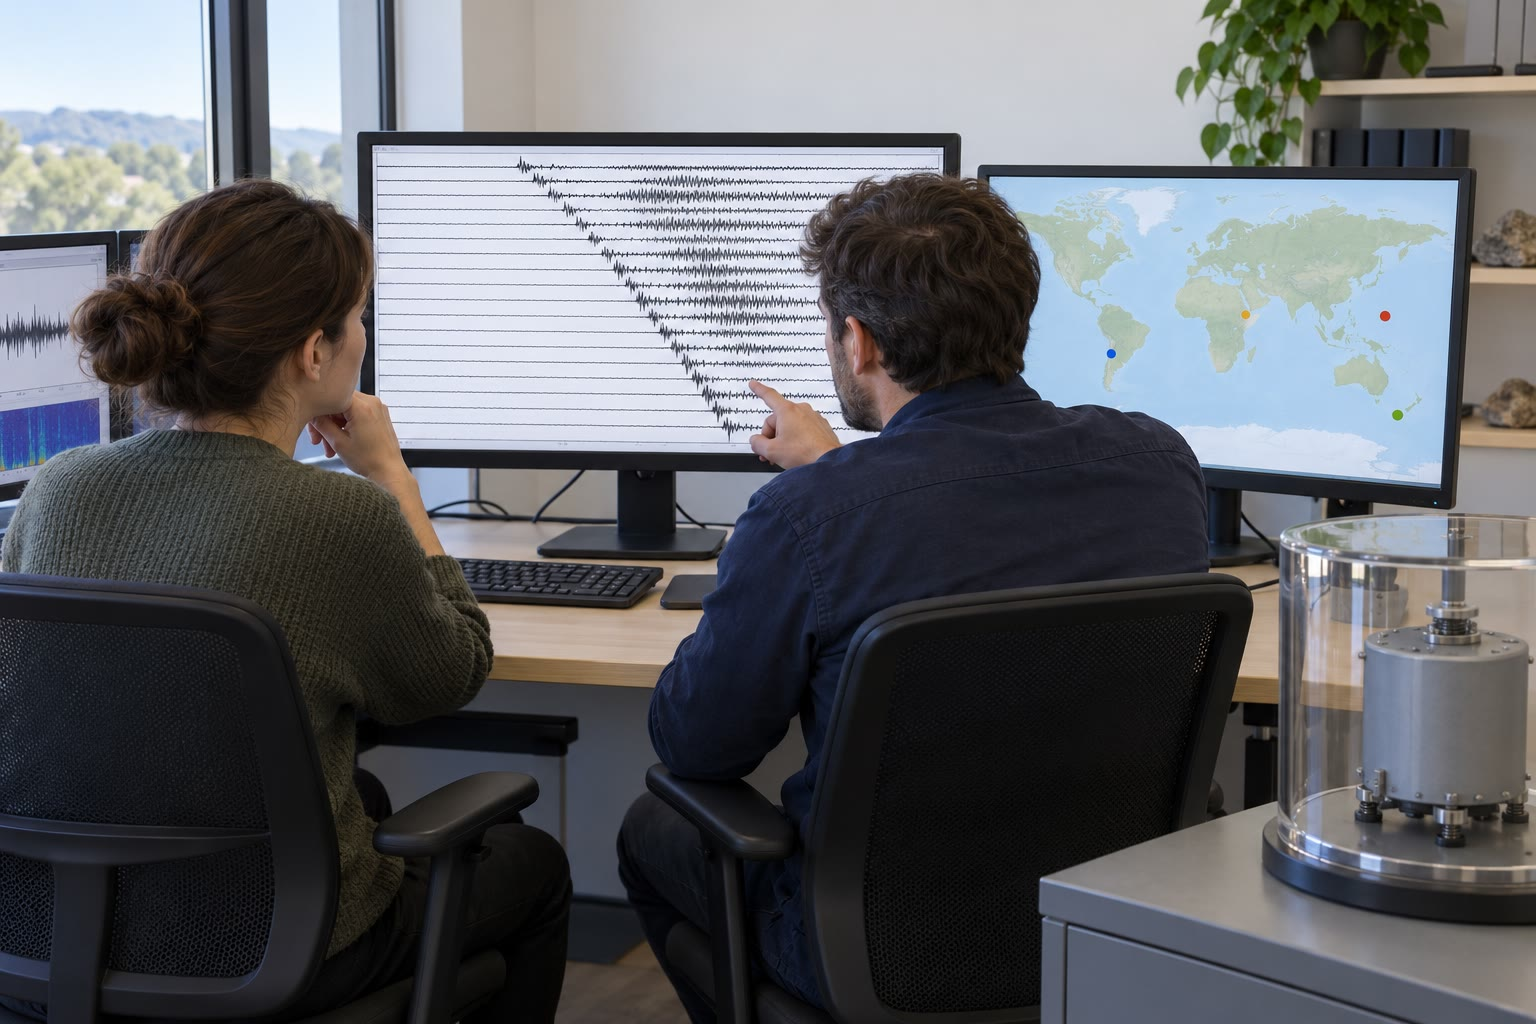
\includegraphics[width=\linewidth]{images/book3/ai/b1-seismic-analysis.jpg}

{\scriptsize भूकंप-विज्ञानी एक अभिलेख-खंड पढ़ते हुए, एक भूकंप के अनुरेख दूरी के अनुसार छाँटे गए स्टेशनों पर (AI से बनाया गया चित्र)।}
\end{minipage}
\end{inthelab}
% ledger: yvo:beachball

\section{भार का मापन: भू-आकलन}\label{sec:b1:earthquake-source:geodesy}

भूकंपों के बीच, एक अवरुद्ध भ्रंश भूकंपमापियों के लिए अदृश्य होता है, पर उसके चारों ओर की ज़मीन चलती है। उपग्रह-स्थिति निर्धारण के स्थायी स्टेशन वह गति मापते हैं, और उनके वेगों का भ्रंश के आर-पार बदलता तरीका बताता है कि वह कितना गहरा अवरुद्ध है।

\begin{definition}[अवरोधन-गहराई]
\label{def:b1:earthquake-source:locking-depth}
किसी भ्रंश की \emph{अवरोधन-गहराई}\index{अवरोधन-गहराई} वह गहराई है जिस तक वह भूकंपों के बीच अवरुद्ध रहता है, उसके नीचे का भ्रंश दीर्घकालिक दर पर स्थिरता से सरकता हुआ; वह उस भ्रंश-भाग की गहराई है जो अगले भूकंप में सरकेगा।
\end{definition}
% ledger: usgs:pp1515-thatcher

\begin{proposition}[एक सरकते भ्रंश के आर-पार अंतर-भूकंपीय वेग]
\label{prop:b1:earthquake-source:interseismic}
मान लीजिए एक प्रत्यास्थ अर्ध-अंतरिक्ष में एक ऊर्ध्वाधर \omterm{def:b1:faults-folds-fabrics:fault-types}{स्ट्राइक-स्लिप भ्रंश} सतह से गहराई $D$ तक अवरुद्ध है, और उसके नीचे दर $V$ पर सरकता है। भ्रंश के समांतर सतह का वेग, उससे दूरी $x$ पर, है
\[
  v(x) = \frac{V}{\pi}\arctan\frac{x}{D} .
\]
यदि भ्रंश तब एक भूकंप में $s$ सरकता है, सतह से गहराई $D$ तक, तो सतह $u(x) = (s/\pi)\arctan(D/x)$ के अनुसार $x > 0$ के लिए विस्थापित होती है, और $-u(-x)$ के अनुसार $x < 0$ के लिए।
\end{proposition}
\admitted

सेवेज और बर्फ़ोर्ड के कारण यह मॉडल \omterm{def:b1:earthquake-source:seismic-cycle}{प्रत्यास्थ प्रतिक्षेप} का सबसे सरल रूप है, और पहले चित्र की बाड़ का वक्र यही है। उसके गुण सूत्र से निकलते हैं।

\begin{proposition}[अंतर-भूकंपीय परिच्छेद को पढ़ना]
\label{prop:b1:earthquake-source:profile}
\cref{prop:b1:earthquake-source:interseismic} के मॉडल में:
\begin{enumerate}[label=(\alph*)]
  \item भ्रंश से दूर वेग $\pm V/2$ की ओर प्रवृत्त होता है, दोनों प्लेटें एक-दूसरे के सापेक्ष $V$ पर चलती हुईं;
  \item भ्रंश के आर-पार वेग के परिवर्तन का आधा उसकी दूरी $D$ के भीतर होता है: $v(\pm D) = \pm V/4$;
  \item सतह की कर्तन-विकृति-दर, $\mathrm dv/\mathrm dx$, भ्रंश पर सबसे बड़ी है, जहाँ वह $V/(\pi D)$ के बराबर है;
  \item यदि भ्रंश, समय $t$ के भार के बाद, एक भूकंप में $s = Vt$ सरकता है, तो हर जगह ज़मीन दोनों ओर $\pm s/2$ विस्थापित होकर रह जाती है: चक्र कोई स्थायी मोड़ नहीं छोड़ता, केवल भ्रंश पर विस्थापन $s$।
\end{enumerate}
\end{proposition}

\begin{proof}
(a) $\arctan(x/D) \to \pm\pi/2$ जब $x \to \pm\infty$। (b) $\arctan 1 = \pi/4$, इसलिए $v(D) = V/4$, और $v$ विषम है। (c) $\mathrm dv/\mathrm dx = (V/\pi D)/(1 +
x^2/D^2)$, जो $x = 0$ पर सबसे बड़ा है। (d) $x > 0$ के लिए, भार ने ज़मीन को $t\,v(x) = (s/\pi)\arctan(x/D)$ और भूकंप ने $(s/\pi)\arctan(D/x)$ से हिलाया; चूँकि $\arctan y + \arctan(1/y) = \pi/2$, $y > 0$ के लिए, योग $s/2$ है। $x < 0$ के लिए चिह्न उलटे हुए वही होता है।
\end{proof}

उपधारणा (b) से \omterm{def:b1:earthquake-source:locking-depth}{अवरोधन-गहराई} स्टेशनों की एक परिच्छेद से मिलती है: वह भ्रंश से वह दूरी है जिस पर वेग, भ्रंश पर अपने मान से, $V$ के एक चौथाई से बदल गया है। एक उथला अवरोधन विकृति को भ्रंश के निकट केंद्रित करता है (नीचे का चित्र), एक गहरा उसे एक चौड़े पट्टे में फैलाता है। सैन एंड्रियास तंत्र के साथ, भू-आकलन से पाई गई अवरोधन-गहराइयाँ विसर्पी खंडों पर लगभग 0 से लेकर \qty{26}{km} तक हैं, और भूकंपों की गहराइयों से मेल खाती हैं: अवरुद्ध भाग वही \omterm{def:b1:stress-strain-rheology:strength-envelope}{भूकंप-जनक परत} है जो \cref{ch:b1:stress-strain-rheology} में है। \qty{34}{mm.yr^{-1}} के सरकन-दर और \qty{15}{km} की \omterm{def:b1:earthquake-source:locking-depth}{अवरोधन-गहराई} के लिए, भ्रंश पर कर्तन-विकृति-दर $\num{0.034}/(\pi\times\num{15000}) = \num{7.2e-7}$ प्रति वर्ष है, जो भ्रंश के आर-पार की एक रेखा को प्रति वर्ष प्रति किलोमीटर एक मिलीमीटर से कम मोड़ती है, फिर भी दो सदियों में एक महान भूकंप के कई मीटर सरकन को संचित करती है।
% ledger: sk:mu-locking, usgs:pp1515-wallace, usgs:pp1515-thatcher

\begin{omfigure}
\begin{tikzpicture}[font=\small]
\begin{axis}[omrecord, width=11cm, height=5.6cm, xmin=-100, xmax=100, ymin=-19, ymax=19,
    xlabel={भ्रंश से दूरी $x$ (km)}, ylabel={वेग $v$ (\unit{mm.yr^{-1}})},
    legend style={font=\scriptsize, at={(0.02,0.96)}, anchor=north west}, legend cell align=left]
  \addplot[omDef, line width=0.9pt, dashed] table[x=x, y=v5] {figdata/out/bachelor-1-interseismic-profiles.dat};
  \addplot[omThm, line width=1.1pt] table[x=x, y=v15] {figdata/out/bachelor-1-interseismic-profiles.dat};
  \addplot[omProp, line width=0.9pt, dotted] table[x=x, y=v25] {figdata/out/bachelor-1-interseismic-profiles.dat};
  \legend{$D = \qty{5}{km}$, $D = \qty{15}{km}$, $D = \qty{25}{km}$}
  \draw[black!50, dashed] (axis cs:-100,17) -- (axis cs:100,17);
  \draw[black!50, dashed] (axis cs:-100,-17) -- (axis cs:100,-17);
  \node[anchor=north west, font=\scriptsize] at (axis cs:-30,17) {$+V/2$};
  \node[anchor=south west, font=\scriptsize] at (axis cs:30,-17) {$-V/2$};
  \draw[black!60] (axis cs:0,-19) -- (axis cs:0,19);
  \node[anchor=east, font=\scriptsize] at (axis cs:-1,5) {भ्रंश};
\end{axis}
\end{tikzpicture}
\par\smallskip{\small एक अवरुद्ध \omterm{def:b1:faults-folds-fabrics:fault-types}{स्ट्राइक-स्लिप भ्रंश} के समांतर ज़मीन का वेग, भ्रंश-रेखा के सापेक्ष, सरकन-दर $V = \qty{34}{mm.yr^{-1}}$ के लिए, जो वैलेस क्रीक पर सैन एंड्रियास भ्रंश की है, और तीन अवरोधन-गहराइयों के लिए (\cref{prop:b1:earthquake-source:interseismic})। अवरोध जितना उथला होगा, वेग के बदलने का पट्टा उतना ही संकरा।}
\label{fig:b1:earthquake-source:interseismic}
\end{omfigure}
% ledger: usgs:pp1515-wallace

उपग्रह-स्थिति निर्धारण कुछ स्टेशनों पर ज़मीन मापता है। रडार उपग्रह उसे हर जगह मापते हैं: एक ही कक्षा से अलग-अलग समयों पर लिए गए एक ही क्षेत्र के दो रडार-चित्र तरंग-दर-तरंग तुलना किए जाते हैं, और कला का अंतर ज़मीन और उपग्रह के बीच की दूरी के परिवर्तन को बिंदु-दर-बिंदु, सौ मीटर के अंतर पर, मानचित्रित करता है, बिना किसी पूर्व-स्थापित स्टेशन-जाल के। एक बड़े कैलिफ़ोर्निया भूकंप, 1992, का पहला ऐसा मानचित्र उसका सह-भूकंपीय विस्थापन एक चित्र में दिखाता था और क्षेत्र में और सर्वेक्षण द्वारा मापे सरकन से मेल खाता था; यह तकनीक, रडार इंटरफ़ेरोमेट्री, पुस्तक 5 से संबंधित है।
% ledger: massonnet:1993

\section{कितनी बार: गुटेनबर्ग–रिक्टर नियम}\label{sec:b1:earthquake-source:gr}

छोटे भूकंप बड़े भूकंपों से कहीं अधिक आम हैं, और एक उल्लेखनीय रूप से नियमित ढंग से।

\begin{proposition}[गुटेनबर्ग–रिक्टर नियम]
\label{prop:b1:earthquake-source:gutenberg-richter}
किसी क्षेत्र और अवधि में\index{गुटेनबर्ग–रिक्टर नियम}, भूकंपों की संख्या $N$, जिनका परिमाण कम से कम $M$ है, इस प्रकार है
\[
  \log_{10} N = a - bM ,
\]
हर $M$ के लिए जो सूची की \omterm{def:b1:earthquake-source:b-value}{पूर्णता-परिमाण} से ऊपर है, स्थिरांकों $a$ और $b$ के साथ, जो क्षेत्र पर निर्भर हैं; अधिकांश सक्रिय क्षेत्रों में $b$, 1 के निकट है।
\end{proposition}
\admitted
% ledger: fd:1993, gr:1944

यह नियम प्रेक्षण का परिणाम है, जिसे बेनो गुटेनबर्ग और चार्ल्स रिक्टर ने 1944 में कैलिफ़ोर्निया के लिए प्रकाशित किया और तब से हर जगह पाया गया; कोई सिद्धांत अभी तक इसे, या $b$ के मान को, व्युत्पन्न नहीं करता।
% ledger: gr:1944

\begin{definition}[b-मान, पूर्णता-परिमाण]
\label{def:b1:earthquake-source:b-value}
किसी क्षेत्र के \omterm{prop:b1:earthquake-source:gutenberg-richter}{गुटेनबर्ग–रिक्टर नियम} का स्थिरांक $b$ उसका \emph{b-मान}\index{b-मान} है। किसी सूची का \emph{पूर्णता-परिमाण}\index{पूर्णता-परिमाण} वह सबसे छोटा परिमाण है जिससे ऊपर वह क्षेत्र और अवधि का हर भूकंप दर्ज करती है।
\end{definition}

1 का \omterm{def:b1:earthquake-source:b-value}{b-मान} हर परिमाण-इकाई के लिए दस गुना कम भूकंप का अर्थ है। \omterm{def:b1:earthquake-source:b-value}{पूर्णता-परिमाण} से नीचे, गिनती रेखा से नीचे रहती है, क्योंकि छोटे भूकंप इतने कम स्टेशनों पर दर्ज होते हैं कि उनके स्थान निर्धारित नहीं हो सकते: नियम मुड़ा हुआ लगता है, और $b$ उसके ऊपर मापा जाना चाहिए। पूरी पृथ्वी के लिए, उथले, मध्यवर्ती और गहरे भूकंपों में बाँटकर, मापे गए मान 0.72 और 1.34 के बीच हैं, परंतु वे एक सूची, परिमाण-परास या विधि से दूसरी में \qty{30}{\percent} या अधिक भिन्न होते हैं: 1 से दूर का मान पहले सूची की जाँच का एक कारण है।
% ledger: fd:1993

\begin{omfigure}
\begin{tikzpicture}[font=\small]
\begin{axis}[omrecord, width=6.4cm, height=5.8cm, ymode=log, xmin=5.8, xmax=9.3, ymin=0.01, ymax=300,
  xlabel={परिमाण $M$}, ylabel={परिमाण $\ge M$ वाली घटनाएँ प्रति वर्ष},
    log basis y=10, title={(a) आवृत्ति और परिमाण}, title style={font=\small}]
  \addplot[omProp, line width=0.9pt, domain=5.8:9.3] table[x=M, y=rate] {figdata/out/bachelor-1-gutenberg_richter-fit.dat};
  \addplot[only marks, mark=*, mark size=1.3pt, omDef] table[x=M, y=rate] {figdata/out/bachelor-1-gutenberg_richter-counts.dat};
  \draw[black!50, dashed] (axis cs:7.5,0.01) -- (axis cs:7.5,300);
  \node[anchor=south west, font=\scriptsize, omProp] at (axis cs:8.45,0.5) {$b = 1.01$};
  \node[anchor=north west, font=\scriptsize, align=left] at (axis cs:7.55,200) {$6.0 \le M \le 7.5$ के लिए\\ निर्धारित};
\end{axis}
\begin{axis}[omrecord, at={(7.6cm,0)}, width=6.4cm, height=5.8cm, xmin=5.8, xmax=9.3, ymin=0, ymax=1.05,
    xlabel={परिमाण $M$}, ylabel={परिमाण $\ge M$ वाली घटनाओं से आघूर्ण का भाग},
    title={(b) आघूर्ण कहाँ जाता है}, title style={font=\small}]
  \addplot[const plot, omDef, line width=0.9pt] table[x=M, y=share] {figdata/out/bachelor-1-gutenberg_richter-moment.dat};
\end{axis}
\end{tikzpicture}
\par\smallskip{\small विश्व के \num{7031} भूकंप, जिनका परिमाण 6 या उससे अधिक है, 1976–2025 (संयुक्त राज्य भूवैज्ञानिक सर्वेक्षण की सूची)। (a) परिमाण कम से कम $M$ वाले भूकंपों की वार्षिक संख्या; रेखा $\log_{10} N$ का $M$ के विरुद्ध न्यूनतम-वर्ग आरोपण है, 6.0 से 7.5 तक, जहाँ हर गिनती 200 से अधिक है: $\log_{10} N = 8.20 - 1.01\,M$ प्रति वर्ष। 8 से ऊपर की थोड़ी-सी घटनाएँ रेखा से नीचे गिरती हैं। (b) कम से कम $M$ परिमाण वाले भूकंपों द्वारा मुक्त कुल \omterm{def:b1:earthquake-source:moment}{भूकंपीय आघूर्ण} का भाग, हर आघूर्ण $10^{1.5M + 9.1}$\,\unit{N.m} से परिकलित: 8 या उससे अधिक परिमाण के 40 भूकंपों ने उसका \qty{63}{\percent} मुक्त किया।}
\label{fig:b1:earthquake-source:gutenberg-richter}
\end{omfigure}
% ledger: data:usgs-comcat (fit and shares computed in figdata/bachelor-1/gutenberg_richter.py)

चित्र की विश्व सूची के लिए, $a = 8.20$ और $b = 1.01$ वाला नियम 7 या उससे अधिक परिमाण के 14 भूकंप प्रति वर्ष पूर्वानुमानित करता है, जैसा प्रेक्षित है, और 8 या उससे अधिक परिमाण के 1.35; जबकि पचास वर्षों में 40, यानी 0.8 प्रति वर्ष, दर्ज हुए। क्या सबसे बड़े भूकंप सचमुच रेखा से कम हैं, जैसा भ्रंशों का परिमित आकार सुझाता, या बस इतने दुर्लभ हैं कि पचास वर्षों से छूट गए, यह इतनी कम घटनाओं से तय नहीं होता। इस सूची में लगभग हर नौवें परिमाण का एक पृष्ठ-तरंग या काय-तरंग परिमाण है, जो संतृप्त होते हैं; सबसे बड़ी घटनाओं के सभी \omterm{def:b1:earthquake-source:mw}{आघूर्ण परिमाण} हैं।
% ledger: data:usgs-comcat

कम परिमाण के असंख्य छोटे भूकंप कम काम करते हैं। उनकी संख्या हर परिमाण-इकाई कम होने पर दस गुना बढ़ती है, परंतु उनके आघूर्ण 31.6 गुना घटते हैं।

\begin{proposition}[सबसे बड़े भूकंप अधिकांश आघूर्ण मुक्त करते हैं]
\label{prop:b1:earthquake-source:largest}
मान लीजिए भूकंप $b < 1.5$ के साथ \omterm{prop:b1:earthquake-source:gutenberg-richter}{गुटेनबर्ग–रिक्टर नियम} का पालन करते हैं, एक सबसे बड़े परिमाण $M_{\max}$ तक, और मान लीजिए वे परिमाण की एक-एक इकाई चौड़े खानों में समूहित हैं, सबसे ऊपर का खाना $M_{\max}$ पर समाप्त होता है। तब सबसे ऊपर के खाने के भूकंप कुल आघूर्ण के भाग $1 - 10^{-(1.5 - b)}$ से अधिक मुक्त करते हैं, चाहे गिने गए सबसे छोटे परिमाण कितने भी छोटे हों: $b = 1$ के लिए \qty{68}{\percent} से अधिक।
\end{proposition}

\begin{proof}
परिमाण के खानों को $k = 0, 1, \dots, K$ से सबसे छोटे से गिनिए, खाना $k$ $M_k$ से $M_k + 1$ तक चलता है, और $M_{k+1} = M_k + 1$। नियम से, खाना $k$ में भूकंपों की संख्या $10^{a - bM_k} - 10^{a - b(M_k+1)} =
10^{a - bM_k}(1 - 10^{-b})$ है; \cref{prop:b1:earthquake-source:moment-steps} से हर एक का आघूर्ण $10^{1.5M_k + 9.1}$ और उसके $10^{1.5}$ गुना के बीच है, और चूँकि हर खाना पिछले का एक इकाई खिसका हुआ है, खाना $k$ का आघूर्ण $C q^k$ है, जहाँ $C$ एक स्थिरांक है, और अनुपात $q = 10^{-b}\times10^{1.5} = 10^{1.5 - b} > 1$।
\[
  S = C(1 + q + \dots + q^K) = C\,\frac{q^{K+1} - 1}{q - 1} ,
\]
और सबसे ऊपर के खाने का भाग है
\[
  \frac{C q^K}{S} = \frac{q^K (q - 1)}{q^{K+1} - 1}
  > \frac{q^K (q - 1)}{q^{K+1}} = 1 - \frac1q = 1 - 10^{-(1.5 - b)} .
\]
$b = 1$ के लिए, $1 - 10^{-0.5} = 0.684$।
\end{proof}

विश्व सूची में भाग इसी क्रम का है: सबसे ऊपर की परिमाण-इकाई, 8.1 से 9.1 तक, पचास वर्षों के आघूर्ण के आधे से अधिक मुक्त करती है, और दो सबसे बड़े भूकंप, 2004 का सुमात्रा–अंडमान और 2011 का तोहोकू, दोनों 9.1 परिमाण के, उसका \qty{29}{\percent} अकेले मुक्त करते हैं। एक प्लेट-सीमा को जो आघूर्ण मुक्त करना है वह उसकी सरकन-दर से तय होता है; प्रस्ताव कहता है कि वह लगभग पूरा उसके सबसे बड़े भूकंपों में मुक्त होता है, और कि अनेक छोटे भूकंप, चाहे कितने भी बार-बार आएँ, भ्रंश को अगले महान भूकंप से मुक्त नहीं करते।
% ledger: data:usgs-comcat, usgs:sumatra-mt, usgs:tohoku-mt

\section{अभ्यास}

\begin{exercise}[$\star$]
\label{exo:b1:earthquake-source:1}
(a) \qty{4e17}{N.m} के \omterm{def:b1:earthquake-source:moment}{भूकंपीय आघूर्ण} वाले भूकंप का \omterm{def:b1:earthquake-source:mw}{आघूर्ण परिमाण} परिकलित कीजिए। (b) तोहोकू भूकंप का $M_0 = \qty{5.59e22}{N.m}$ था: उसका परिमाण जाँचिए। (c) परिमाण 7.0 वाले भूकंप का \omterm{def:b1:earthquake-source:moment}{भूकंपीय आघूर्ण} क्या है?
% ledger: usgs:tohoku-mt
\end{exercise}

\begin{exercise}[$\star$]
\label{exo:b1:earthquake-source:2}
एक \omterm{def:b1:faults-folds-fabrics:fault-types}{स्ट्राइक-स्लिप भ्रंश} \qty{25}{mm.yr^{-1}} पर भारित है, और उसके भूकंप हर बार लगभग \qty{3}{m} सरकते हैं। (a) यदि वे उनके बीच पूरी तरह अवरुद्ध है, तो उनका \omterm{def:b1:earthquake-source:seismic-cycle}{पुनरावृत्ति अंतराल} क्या है? (b) और यदि सरकन-दर का आधा स्थिर विसर्पण से लिया जाता है?
\end{exercise}

\begin{exercise}[$\star$]
\label{exo:b1:earthquake-source:3}
परिमाण 7.4 वाले भूकंप का \omterm{def:b1:earthquake-source:moment}{भूकंपीय आघूर्ण} परिमाण 6.2 वाले से कितने गुना बड़ा है? परिमाण 6.2 के कितने भूकंप वही आघूर्ण मुक्त करेंगे?
\end{exercise}

\begin{exercise}[$\star$]
\label{exo:b1:earthquake-source:4}
एक क्षेत्र में, $b = 1$ के साथ, हर वर्ष परिमाण 3 या उससे अधिक के एक हज़ार भूकंप दर्ज होते हैं। हर वर्ष परिमाण 5 या उससे अधिक, और परिमाण 6 या उससे अधिक के कितने अपेक्षित हैं? परिमाण 7 या उससे अधिक के भूकंपों के बीच औसत समय क्या है?
\end{exercise}

\begin{exercise}[$\star\star$]
\label{exo:b1:earthquake-source:5}
1906 के भूकंप ने सैन एंड्रियास भ्रंश को लगभग \qty{430}{km} पर तोड़ा। (a) मानकर कि भंजन \qty{15}{km} गहराई तक पहुँचा, \qty{4}{m} के औसत सरकन के साथ, और $\mu = \qty{30}{GPa}$, उसका \omterm{def:b1:earthquake-source:moment}{भूकंपीय आघूर्ण} और \omterm{def:b1:earthquake-source:mw}{आघूर्ण परिमाण} परिकलित कीजिए। (b) यदि भंजन केवल \qty{10}{km} गहरा था तो परिमाण कितना बदलता है? (c) दोनों अनुमानों में से कौन-सा 7.9 के निकट है?
% ledger: pp1515:1906, usgs:hist-mw
\end{exercise}

\begin{exercise}[$\star\star$]
\label{exo:b1:earthquake-source:6}
तोहोकू भूकंप का भंजन लगभग \qty{400}{km} लंबा और \qty{150}{km} चौड़ा था, और उसका आघूर्ण \qty{5.59e22}{N.m} था। (a) $\mu = \qty{30}{GPa}$ के साथ उसका औसत सरकन परिकलित कीजिए। (b) प्रशांत प्लेट लगभग \qty{83}{mm.yr^{-1}} पर जापान के नीचे धँसती है: यदि अंतरापृष्ठ पूरी तरह अवरुद्ध है, तो यह सरकन जमा होने में कितना समय लेता है? (c) और यदि अवरोधित भाग 0.8 है, या 0.5?
% ledger: usgs:tohoku-mt, usgs:tohoku-summary
\end{exercise}

\begin{exercise}[$\star\star$]
\label{exo:b1:earthquake-source:7}
2004 के सुमात्रा–अंडमान भूकंप का एक \omterm{def:b1:earthquake-source:focal-mechanism}{नोडल तल} \omterm{def:b1:geological-maps:attitude}{स्ट्राइक} $329$, \omterm{def:b1:geological-maps:attitude}{नति} \ang{8} और \omterm{def:b1:faults-folds-fabrics:fault-elements}{रेक} \ang{110} रखता है। (a) $\mathbf n$ और $\mathbf d$ को पूर्व, उत्तर और ऊपर के घटकों में लिखिए। (b) \omterm{def:b1:earthquake-source:focal-mechanism}{सहायक तल} का \omterm{def:b1:geological-maps:attitude}{स्ट्राइक}, \omterm{def:b1:geological-maps:attitude}{नति} और \omterm{def:b1:faults-folds-fabrics:fault-elements}{रेक} ज्ञात कीजिए। (c) P और T अक्षों की दिगंश और अवनति ज्ञात कीजिए। (d) कौन-सा तल भ्रंश है, और वह किस प्रकार का भ्रंश है?
% ledger: usgs:sumatra-mt
\end{exercise}

\begin{exercise}[$\star\star$]
\label{exo:b1:earthquake-source:8}
एक ऊर्ध्वाधर भ्रंश जो $045$ \omterm{def:b1:geological-maps:attitude}{स्ट्राइक} करता है, \omterm{def:b1:faults-folds-fabrics:fault-types}{दाएँ-पार्श्वीय} सरकता है। (a) उद्गम से क्षैतिज रूप से उत्तर, पूर्व, दक्षिण और पश्चिम की ओर के स्टेशनों की ओर निकली तरंगों के लिए, कौन-सी धक्कों के रूप में पहुँचती हैं और कौन-सी खिंचाव के रूप में? (b) P और T अक्षों की दिगंश दीजिए। (c) दिखाइए कि $135$ \omterm{def:b1:geological-maps:attitude}{स्ट्राइक} करते ऊर्ध्वाधर तल पर एक \omterm{def:b1:faults-folds-fabrics:fault-types}{बाएँ-पार्श्वीय} सरकन वही प्रथम गतियाँ देता है।
\end{exercise}

\begin{exercise}[$\star\star$]
\label{exo:b1:earthquake-source:9}
एक अवरुद्ध \omterm{def:b1:faults-folds-fabrics:fault-types}{स्ट्राइक-स्लिप भ्रंश} के आर-पार, दोनों ओर के दूर-क्षेत्र स्टेशन एक-दूसरे के सापेक्ष \qty{40}{mm.yr^{-1}} पर चलते हैं। भ्रंश से \qty{10}{km} पर एक स्टेशन भ्रंश-रेखा के सापेक्ष \qty{10}{mm.yr^{-1}} पर चलता है। (a) \omterm{def:b1:earthquake-source:locking-depth}{अवरोधन-गहराई} ज्ञात कीजिए। (b) भ्रंश से \qty{30}{km} पर एक स्टेशन के वेग का पूर्वानुमान कीजिए। (c) भ्रंश पर कर्तन-विकृति-दर परिकलित कीजिए।
\end{exercise}

\begin{exercise}[$\star\star\star$]
\label{exo:b1:earthquake-source:10}
(a) दिखाइए कि यदि $b$ 1.5 से बड़ा होता, तो किसी क्षेत्र के भूकंपों का कुल आघूर्ण सबसे छोटे भूकंपों से प्रभुत्व में होता। (b) $b = 0.8$ के लिए, सबसे ऊपर की परिमाण-इकाई कम से कम कितना आघूर्ण मुक्त करती है? (c) विश्व सूची के $a = 8.20$ और $b = 1.01$ प्रति वर्ष के साथ, नियम पचास वर्षों में परिमाण 9 या उससे अधिक के कितने भूकंप पूर्वानुमानित करता है? 1976–2025 की सूची में दो हैं; टिप्पणी कीजिए।
% ledger: data:usgs-comcat
\end{exercise}

\begin{exercise}[$\star\star\star$]
\label{exo:b1:earthquake-source:11}
एक सीधी बाड़ एक अवरुद्ध \omterm{def:b1:faults-folds-fabrics:fault-types}{दाएँ-पार्श्वीय} भ्रंश के आर-पार $V =
\qty{34}{mm.yr^{-1}}$ और $D = \qty{15}{km}$ के साथ बनाई गई है। (a) 150 वर्ष बाद, भ्रंश से पूर्व में \qty{1}{km}, \qty{15}{km} और \qty{50}{km} पर स्थित खंभे, भ्रंश पर के खंभे के सापेक्ष, उसके अनुदिश कितने चले हैं? (b) भ्रंश फिर एक भूकंप में पूरे घाटे के बराबर सरकता है। सरकन क्या है, और भूकंप के दौरान तीनों खंभों में से हर एक कितना चलता है? (c) भाग (d) का \cref{prop:b1:earthquake-source:profile} तीन खंभों पर जाँचिए।
% ledger: usgs:pp1515-wallace
\end{exercise}

\begin{exercise}[$\star\star\star$]
\label{exo:b1:earthquake-source:12}
एक भूकंप की एक क्षैतिज \omterm{def:b1:earthquake-source:focal-mechanism}{P-अक्ष} है जिसकी दिगंश $000$ है, और एक क्षैतिज \omterm{def:b1:earthquake-source:focal-mechanism}{T-अक्ष} जिसकी दिगंश $090$ है। (a) दिखाइए कि उसके \omterm{def:b1:earthquake-source:focal-mechanism}{नोडल तल} ऊर्ध्वाधर हैं और $045$ तथा $135$ \omterm{def:b1:geological-maps:attitude}{स्ट्राइक} करते हैं, $\mathbf n$ और $\mathbf d = (\mathbf T \pm \mathbf P)/\sqrt2$ का उपयोग करते हुए। (b) हर तल पर सरकन की संवेदना दीजिए। (c) यदि भ्रंश $\phi = \ang{30}$ वाली चट्टान में एक नए भ्रंश के रूप में बना होता, \omterm{def:b1:earthquake-source:focal-mechanism}{P-अक्ष} के अनुदिश एक $\sigma_1$ के अंतर्गत, तो वह किन स्ट्राइकों पर होता, और \omterm{def:b1:earthquake-source:focal-mechanism}{P-अक्ष} $\sigma_1$ का केवल सन्निकटन क्यों है? (d) पास में एक मानचित्रित भ्रंश $040$ \omterm{def:b1:geological-maps:attitude}{स्ट्राइक} करता है। कौन-सा \omterm{def:b1:earthquake-source:focal-mechanism}{नोडल तल} संभवतः भ्रंश है, और उसके सरकन की संवेदना क्या है?
\end{exercise}

\section{समस्या: एक अवरुद्ध भ्रंश पर अगला महान भूकंप}

\begin{problem}[{सप्ताहांत समस्या --- एक स्ट्राइक-स्लिप प्लेट-सीमा का एक अवरुद्ध खंड, उसके भार और पिछले भूकंपों से अगले भूकंप के परिमाण तक}]
\label{pb:b1:earthquake-source:1}
% values: calc/ch18.py; an invented fault (the numbers are of a realistic order)
एक सीधा, ऊर्ध्वाधर \omterm{def:b1:faults-folds-fabrics:fault-types}{स्ट्राइक-स्लिप भ्रंश} दो प्लेटों के बीच की सीमा बनाता है। उसका एक \qty{250}{km} लंबा खंड अवरुद्ध है; उसके भूकंप \qty{15}{km} से गहरे शुरू नहीं होते। उसके आर-पार खोदी गई खंदकें उसके अंतिम चार महा-भूकंपों को लगभग 1050, 1290, 1480 और 1712 की तिथि देती हैं, जिनके विस्थापन \num{7.0}, \num{6.0}, \num{5.5} और \qty{7.5}{m} हैं। दोनों ओर भ्रंश से दूर के स्थायी स्टेशन एक-दूसरे के सापेक्ष \qty{30}{mm.yr^{-1}} पर चलते हैं। $\mu =
\qty{30}{GPa}$ लीजिए, वर्ष 2025 को वर्तमान मानिए, और परिमाण 0.01 तक दीजिए।

\medskip
\noindent\textbf{भाग I --- भार।}
\begin{enumerate}
  \item चार भूकंपों के बीच के अंतराल और उनका औसत परिकलित कीजिए।
  \item औसत विस्थापन परिकलित कीजिए, और पूरी तरह अवरुद्ध भ्रंश के लिए \cref{prop:b1:earthquake-source:recurrence} से उसके द्वारा निहित \omterm{def:b1:earthquake-source:seismic-cycle}{पुनरावृत्ति अंतराल}।
  \item केवल खंदक से सरकन-दर परिकलित कीजिए, अंतिम तीन भूकंपों के विस्थापनों और पहले तथा अंतिम के बीच के समय से। भू-आकलन की दर से तुलना कीजिए।
  \item अंतिम भूकंप कितने समय पहले था, और यदि खंड पूरी तरह अवरुद्ध है तो तब से कितना सरकन-घाटा जमा हुआ है?
  \item इस घाटे की खंदक के विस्थापनों से तुलना कीजिए। क्या अगला भूकंप समय से पहले आना चाहिए था?
  \item खंदक अगले भूकंप की तिथि क्यों नहीं दे सकती?
\end{enumerate}

\medskip
\noindent\textbf{भाग II --- अगले भूकंप का आकार।}
\begin{enumerate}[resume]
  \item भ्रंश-खंड के अवरुद्ध भाग का क्षेत्रफल क्या है?
  \item वह \omterm{def:b1:earthquake-source:moment}{भूकंपीय आघूर्ण} परिकलित कीजिए जो पूरा घाटा मुक्त करेगा।
  \item 1712 के भूकंप का \omterm{def:b1:earthquake-source:mw}{आघूर्ण परिमाण} परिकलित कीजिए, यह मानकर कि उसने वही क्षेत्र तोड़ा, जिसका औसत सरकन उसका खंदक-विस्थापन था।
  \item अगले भूकंप का आघूर्ण 1712 के आघूर्ण से कितने गुना अधिक है, और वह परिमाण की कितनी इकाइयाँ है?
  \item यदि खंड का केवल आधा उसी सरकन के साथ टूटा, तो परिमाण क्या होगा?
  \item खंड हर वर्ष कितना \omterm{def:b1:earthquake-source:moment}{भूकंपीय आघूर्ण} संचित करता है?
\end{enumerate}

\medskip
\noindent\textbf{भाग III --- आवृत्ति और ऊर्जा।}
\begin{enumerate}[resume]
  \item क्षेत्र की सूची $\log_{10} N = 4.3 - M$ प्रति वर्ष का अनुसरण करती है, क्षेत्र के सभी भ्रंशों से। उसका \omterm{def:b1:earthquake-source:b-value}{b-मान} क्या है, और वह हर वर्ष परिमाण 5 या उससे अधिक, और 6 या उससे अधिक के कितने भूकंप देती है?
  \item यह कितना माध्य समय देती है परिमाण 7 या उससे अधिक, और परिमाण 8 या उससे अधिक, के भूकंपों के बीच?
  \item सूची से एक महान भूकंप की पुनरावृत्ति की तुलना खंदक से मिली पुनरावृत्ति से कीजिए। अंतर छोटे भूकंपों के नियम से महान भूकंपों का पूर्वानुमान लगाने के बारे में क्या कहता है?
  \item क्षेत्रीय नियम के परिमाण 5 से 8 तक के भूकंप, सब मिलकर, लगभग \qty{5.5e17}{N.m} प्रति वर्ष मुक्त करते हैं। खंड के आघूर्ण का कितना भाग वह है?
  \item अगला महान भूकंप परिमाण 6 के भूकंप से कितनी गुना अधिक ऊर्जा विकिरित करेगा?
  \item \cref{prop:b1:earthquake-source:largest} का उपयोग करके समझाइए कि खंड के मध्यम भूकंप उसे क्यों मुक्त नहीं करते।
\end{enumerate}

\medskip
\noindent\textbf{भाग IV --- स्टेशनों से अवरोधन-गहराई।}
\begin{enumerate}[resume]
  \item भ्रंश-रेखा के सापेक्ष खंड के आर-पार एक स्टेशन-परिच्छेद, $-11.6$, $-7.5$, $-3.1$, $3.1$, $7.5$ और \qty{11.6}{mm.yr^{-1}} वेग देता है, $x = -40$, $-15$, $-5$, $5$, $15$ और \qty{40}{km} पर। जाँचिए कि परिच्छेद विषम है, और भ्रंश से दूर अपेक्षित वेग दीजिए।
  \item \qty{15}{km} के स्टेशन से \omterm{def:b1:earthquake-source:locking-depth}{अवरोधन-गहराई} परिकलित कीजिए।
  \item \qty{5}{km} और \qty{40}{km} के स्टेशनों से उसे फिर परिकलित कीजिए, और छोटे अंतरों की व्याख्या कीजिए।
  \item \omterm{def:b1:earthquake-source:locking-depth}{अवरोधन-गहराई} की भूकंपों की गहराई से तुलना कीजिए, और बताइए कि उन्हें क्यों मेल खाना चाहिए।
  \item भ्रंश पर कर्तन-विकृति-दर परिकलित कीजिए।
  \item 0.01 तक, उस भूकंप का \omterm{def:b1:earthquake-source:mw}{आघूर्ण परिमाण} क्या है जो खंड का पूरा सरकन-घाटा मुक्त करेगा?
\end{enumerate}
\end{problem}
